\documentclass[12pt,a4paper]{article}

\newenvironment{sftabbing}[1][1]
  {\par\sffamily#1\tabbing}
  {\endtabbing}
\usepackage[utf8]{inputenc}
\usepackage{amsmath}
\usepackage{amsfonts}
\usepackage{amssymb}
\usepackage[margin = 1in, bottom=1in, top=1in]{geometry}
\usepackage{fancyhdr}
\usepackage{graphicx}
\usepackage{titlesec}
\usepackage{float}
\usepackage{amsmath}
\usepackage[utf8]{inputenc}
\usepackage[english]{babel}
\usepackage{siunitx}
\usepackage{hyperref}
\usepackage[all]{hypcap}
\usepackage[export]{adjustbox}
\usepackage{textcomp}
\usepackage{gensymb}
\usepackage{physics}
\usepackage[nottoc,notlot,notlof]{tocbibind}
\newcommand\tab[1][1cm]{\hspace*{#1}}
\parindent 0ex
\titleformat{\subparagraph}
    {\normalfont\normalsize\bfseries}{\thesubparagraph}{1em}{}
\titlespacing*{\subparagraph}{\parindent}{3.25ex plus 1ex minus .2ex}{.75ex plus .1ex}
\usepackage[acronym,nomain]{glossaries}
\usepackage{slashbox}
\usepackage[acronym]{glossaries}
\usepackage{acronym}
\usepackage{subcaption}
\usepackage{siunitx}
\usepackage{lscape}
\usepackage{listings}

\usepackage{xcolor}

%New colors defined below
\definecolor{codegreen}{rgb}{0,0.6,0}
\definecolor{codegray}{rgb}{0.5,0.5,0.5}
\definecolor{codepurple}{rgb}{0.58,0,0.82}
\definecolor{backcolour}{rgb}{0.95,0.95,0.92}

%Code listing style named "mystyle"
\lstdefinestyle{mystyle}{
  backgroundcolor=\color{backcolour}, commentstyle=\color{codegreen},
  keywordstyle=\color{magenta},
  numberstyle=\tiny\color{codegray},
  stringstyle=\color{codepurple},
  basicstyle=\ttfamily\footnotesize,
  breakatwhitespace=false,         
  breaklines=true,                 
  captionpos=b,                    
  keepspaces=true,                 
  numbers=left,                    
  numbersep=5pt,                  
  showspaces=false,                
  showstringspaces=false,
  showtabs=false,                  
  tabsize=2
}

\colorlet{punct}{red!60!black}
\definecolor{background}{HTML}{EEEEEE}
\definecolor{delim}{RGB}{20,105,176}
\colorlet{numb}{magenta!60!black}

\lstdefinelanguage{json}{
    basicstyle=\normalfont\ttfamily,
    numbers=left,
    numberstyle=\scriptsize,
    stepnumber=1,
    numbersep=8pt,
    showstringspaces=false,
    breaklines=true,
    frame=lines,
    backgroundcolor=\color{background},
    literate=
     *{0}{{{\color{numb}0}}}{1}
      {1}{{{\color{numb}1}}}{1}
      {2}{{{\color{numb}2}}}{1}
      {3}{{{\color{numb}3}}}{1}
      {4}{{{\color{numb}4}}}{1}
      {5}{{{\color{numb}5}}}{1}
      {6}{{{\color{numb}6}}}{1}
      {7}{{{\color{numb}7}}}{1}
      {8}{{{\color{numb}8}}}{1}
      {9}{{{\color{numb}9}}}{1}
      {:}{{{\color{punct}{:}}}}{1}
      {,}{{{\color{punct}{,}}}}{1}
      {\{}{{{\color{delim}{\{}}}}{1}
      {\}}{{{\color{delim}{\}}}}}{1}
      {[}{{{\color{delim}{[}}}}{1}
      {]}{{{\color{delim}{]}}}}{1},
}

\lstset{basicstyle=\ttfamily,
  showstringspaces=false,
  commentstyle=\color{red},
  keywordstyle=\color{blue}
}


\titleformat{\paragraph}
{\normalfont\normalsize\bfseries}{\theparagraph}{1em}{}
\titlespacing*{\paragraph}
{0pt}{3.25ex plus 1ex minus .2ex}{1.5ex plus .2ex}
\setcounter{secnumdepth}{4}
\setcounter{tocdepth}{4}
\makeglossaries 
\renewcommand{\headrulewidth}{0pt}


\fancypagestyle{a}{\fancyhf[L]{\includegraphics[scale=0.25]{1.jpg}}\fancyhead[R]{\includegraphics[scale=1.0]{2.png}}\fancyfoot[]}

\lstset{style=mystyle}
\begin{document}

\begin{titlepage}
\begin{center}
\setcounter{page}{1}

\thispagestyle{a}
\vspace*{2cm}
\large{Faculty of Electrical Engineering and Embedded Systems} \\[4mm]

\line(1,0){450}\\
\Large{\textbf{Analysis and evaluation of needs for a generic and scalable cloud based OTA update system}}\\
\line(1,0){450}\\ [4mm]

\large{\textit{Master Program in Electrical Engineering and Embedded Systems}}\\[6mm] \Large{\textit{Master Thesis}}\\[6mm]

\large{Submitted by:} \\ [4mm]
\large{\textbf{Prithvi Patel}} \\ [1.5cm]

\large{Supervising Professors:} \\ [4mm]
\large{\textbf{Prof. Dr. rer. nat. Markus Pfeil}} \\ [4mm]
\large{\textbf{Prof. Dr.-Ing. Lothar Berger}} \\ [1.5cm]

\large{Industrial Supervisors:} \\ [4mm]
\large{\textbf{Ms. Christina Baur}} \\ [4mm]
\large{\textbf{Mr. Jochen Schaz}} \\ [4mm]
\large{Soluware GmbH} \\ [1.5cm]

\large{Ravensburg, September 2022} \\ [4mm]

\end{center}
\end{titlepage}

\newpage
\pagestyle{fancy}
\fancyfoot{}
\fancyhead{}

\setlength{\footskip=0pt}
\setlength{\headheight=35pt}

\newpage
\section*{Acknowledgement}

Soluware GmbH provided a great deal of support and assistance. The thesis dissertation was completed in the Software Development department. I want to thank Ms. Christina Baur and Mr. Jochen Schaz for providing me the opportunity to write the thesis at Soluware GmbH. Their expertise was invaluable in formulating the research topic, methodology, and thesis structure. Their guidance helped me in my research and thesis writing. \\

I sincerely thank my academic supervisor, Prof. Dr. rer. nat. Markus Pfeil and Prof. Dr.-Ing. Lothar Berger for their insightful comments, constant support, and motivation. A special thanks to my official supervisors, Ms. Christina Baur, and Mr. Jochen Schaz, for their excellent cooperation and technical suggestions during the research work. I want to thank all my colleagues at work for their support and cooperation. \\

\vspace{3cm}

Ravensburg, September 2022


\newpage
\section*{Abstract}

Over-the-Air update systems are becoming an essential part of almost all technological sectors. All the devices must conduct safe operations, from intelligent devices to automotive vehicles. Implementing the individual OTA update systems for all IoT devices can become costly. A company with three different IoT devices for three individual sectors needs three separate infrastructures for the OTA update system. Having a generic OTA update system architecture is beneficial. \\

Along the way, a brief analysis was performed on the OTA update systems for the IoT devices from various sectors. During the analysis phase, the individual scenarios were realized. Based on the scenarios, the architectural design and security criteria were formed. Based on these criteria, the OTA update systems for the devices from various sectors were compared, and the necessary components were fetched from these architectures. The generic and scalable OTA update system architecture was designed based on the components fetched before. \\

A prototype for the architecture was implemented. Raspberry Pi 3B+ is used as an IoT device, Microsoft Azure is the cloud provider, and OpenSSL and WinSCP were used as parts of the Software Deployment client. The generic and scalable OTA update system architecture is evaluated using standardized methods used worldwide in industries. Three methods were considered during the evaluation phase: ATAM, SAAM, and ARID. Each of their steps and necessities was considered. ATAM was chosen for the evaluation based on these considerations. In the end, the final results and future work were described. \\


\newpage
\pagestyle{fancy}
\fancyfoot{}
\fancyhead{}
\setlength{\footskip=25pt}
\setlength{\headheight=0pt}
%\renewcommand{\footrulewidth}{0.4pt}

\fancyfoot{}
\newpage

\rfoot{Page $\vert$ \thepage}
\pagenumbering{roman}
\setcounter{page}{5}
\tableofcontents
\clearpage

\section*{Section with acronyms}

\begin{sftabbing}[\small]
\hspace{6cm}\=\hspace{4.5cm}\=\kill
\textbf{OTA} \> Over the Air \> \\
\textbf{IoT} \> Internet of Things \> \\
\textbf{CPS} \> Cyber-Physical Systems \> \\
\textbf{ECU} \> Electronic Control Unit \> \\
\textbf{ADAS} \> Advanced Driver Assistance System \> \\
\textbf{CAN} \> Controller Area Network \> \\
\textbf{LIN} \> Local Interconnect Network \> \\
\textbf{OEM} \> Original Equipment Manufacturer \> \\
\textbf{ICT} \> Information and Communication Technology \> \\
\textbf{IaaS} \> Infrastructure as a Service \> \\
\textbf{PaaS} \> Platform as a Service \> \\
\textbf{SaaS} \> Software as a Service \> \\
\textbf{API} \> Application Programming Interface \> \\
\textbf{SOA} \> Service Oriented Architecture\> \\
\textbf{ESB} \> Enterprise Service Bus\> \\
\textbf{CQRS} \> Command Query Responsibility Segregation\> \\
\textbf{DES} \> Digital Encryption Standard\> \\
\textbf{AES} \> Advanced Encryption Standard\> \\
\textbf{RSA} \> Rivest, Shamir, Adleman\> \\
\textbf{SHA} \> Secure Hash Algorithm\> \\
\textbf{CA} \> Certificate Authority\> \\
\textbf{PKI} \> Public Key Infrastructure\> \\
\textbf{3G} \> Third Generation\> \\
\textbf{4G} \> Fourth Generation\> \\
\textbf{IEEE} \> Institute of Electrical and Electronics Engineers\> \\
\textbf{DTC} \> Diagnostic Trouble Codes\> \\
\textbf{WVI} \> Wireless Vehicle Interface\> \\
\textbf{OBD} \> On-Board Diagnostics\> \\
\textbf{DT} \> Diagnostic Tester\> \\
\textbf{CGW} \> Central Gateway\> \\
\textbf{FTP} \> File Transfer Protocol\> \\
\textbf{HTTPS} \> HyperText Transfer Protocol Secure\> \\
\textbf{MQTT} \> Message Queuing Telemetry Transport\> \\
\textbf{TLS} \> Transport Layer Security\> \\
\textbf{MCU} \> Microcontroller Unit\> \\
\textbf{RTOS} \> Real-Time Operating System\> \\
\textbf{AWS} \> Amazon Web Service\> \\
\textbf{Wi-Fi} \> Wireless Fidelity\> \\
\textbf{TCP/IP} \> Transmission Control Protocol/ Internet Protocol\> \\
\textbf{SDK} \> Software Development Kit\> \\
\textbf{BLE} \> Bluetooth Low Energy\> \\
\textbf{IAM} \> Identity and Access Management\> \\
\textbf{KB} \> Kilobyte\> \\
\textbf{JTAG} \> Joint Test Action Group\> \\
\textbf{ACM} \> Amazon Certificate Manager\> \\
\textbf{CPU} \> Central Processing Unit\> \\\\
\textbf{PC} \> Personal Computer\> \\
\textbf{EE} \> Electric or Electronics\> \\
\textbf{SOTA} \> Software Over the Update\> \\
\textbf{USB} \> Universal Serial Bus\> \\
\textbf{OMA} \> Open Mobile Alliance\> \\
\textbf{DM} \> Device Management\> \\
\textbf{REST} \> REpresentational State Transfer\> \\
\textbf{OS} \> Operating System\> \\
\textbf{SVM} \> Sensor Virtualization Module\> \\
\textbf{P2P} \> Peer-to-Peer\> \\
\textbf{PAN} \> Personal Area Network\> \\
\textbf{MB} \> Megabyte\> \\
\textbf{GB} \> Gigabyte\> \\
\textbf{SFTP} \> Secure or SSH File Transfer Protocol\> \\
\textbf{SSH} \> Secure SHell\> \\
\textbf{JSON} \> JavaScript Object Notation\> \\
\textbf{ATAS} \> Architecture Trade-off Analysis Method\> \\
\textbf{SAAM} \> Software Architecture Analysis Method\> \\
\textbf{ARID} \> Active Reviews for Intermediate Designs\> \\
\textbf{ARD} \> Admission, Review and Dismissal\> \\
\textbf{DPS} \> Device Provisioning Service\> \\
\textbf{HSM} \> Hardware Security Module\> \\
\textbf{MD5} \> Hardware Security Module\> \\

\end{sftabbing} 

\printglossary[type=\acronymtype]

\newpage

\addcontentsline{toc}{section}{\listfigurename}
\listoffigures
\clearpage


\fancyfoot{}
\rfoot{\thepage}
\pagenumbering{arabic}
\setcounter{page}{1}
\renewcommand{\baselinestretch}{1.5} % line space
\section{Introduction}

This chapter consists of the motivation of the thesis, objectives, research goals, and thesis structure.

\subsection{Motivation}

The software provides many services in modern vehicles and machines today. Therefore, the software update is required to improve security, efficiency, and compatibility. It is possible to update its features and settings wirelessly, and this update method is referred to as Over the Air (OTA). \cite{r1} \\

In the Agriculture sector, the author from \cite{r2} has stated that a single classical OTA architecture cannot fulfill all the requirements for Smart Agriculture, also known as Agriculture 4.0. Moreover, the author added that improving the adaptability, efficiency, and resilience of production systems in agriculture, increasing profit, reasonable allocation of food resources, and avoiding food waste is a few of the requirements of Smart Agriculture. Furthermore, the comparison is essential to highlight the choice for the advantages and disadvantages of generic OTA update system architecture. \\

On the other side, the author from \cite{r3} proposes a generic architecture for wireless updates for the Automobile sector. It offers a generic architecture for wireless updates for the OTA update system, enabling efficient and secure wireless updates for the Automobile embedded systems. \\

Different OTA architectures must be used in various sectors responsible for functioning according to their respective sector's requirements. This research aims to design a new architecture for a generic and scalable cloud-based OTA update system using the architecture proposed in the previous study.

\subsection{Objectives}

The goal of this new architecture for the OTA update system is to function correctly in various sectors according to their requirements. Analyzing the OTA technology is considered the first objective since many researchers are working in this area of research. Moreover, it is required to find the components and technology used to design the architectures from previous studies. It is necessary to use it as a reference for creating a new generic and scalable OTA architecture. The second objective is to design a concept of a generic and scalable architecture for the OTA update system. The third objective is to evaluate the newly designed generic and scalable architecture for the OTA update system and check whether it is feasible according to the prospectives of different sectors using modern evaluation techniques.

\subsection{Reasearch Goals}

This research aims to design a generic and scalable OTA architecture based on Cloud. This generic and scalable OTA architecture should function under various sectors and meet the requirements of multiple sectors. Another research goal is to analyze the need for generic and scalable cloud-based OTA architecture. A simple example would be assuming that a company develops embedded systems for automobile vehicles, home appliances, and smartphones. Suppose the company creates the OTA update system for all three types of embedded systems separately. It will increase the cost and the developer's development and software release management efforts. Applying a generic and scalable OTA update system to all three types of embedded systems is beneficial.


\subsection{Thesis Structure}

The outline of the thesis is as follows: \\

\textbf{Chapter 2 Fundamentals and state-of-the-art} discusses the fundamentals of the Over-the-Air (OTA) Update Mechanism, its requirements, benefits, and a basic procedure of its working. It also discusses the fundamentals of cloud computing, software architecture designing methods, and evaluation techniques. \\

\textbf{Chapter 3 Analysis of existing OTA update systems} discusses the OTA update system from the previous research. It consists of a brief analysis of various sectors' current OTA update system architectures.  \\

\textbf{Chapter 4 Architectural differences of existing OTA update system} discusses the advantages and disadvantages of the OTA update system from previous research. This chapter also briefly compares those architectures and components for the new generic and scalable cloud-based OTA update system architecture design. \\

\textbf{Chapter 5 Designing a generic and scalable OTA architecture concept} describes the new generic and scalable OTA update system architecture based on the cloud. This chapter discusses each new generic and scalable cloud-based OTA update system architecture component. \\

\textbf{Chapter 6 Feasibility of generic and scalable OTA architecture} describes the tools and steps used to implement a prototype for a generic and scalable OTA architecture. \\

\textbf{Chapter 7 Evaluation of the generic and scalable OTA architecture concept} discusses the evaluation of the newly designed architectural concept based on modern techniques mentioned in chapter 2. This chapter also discusses the feasibility of the freshly prepared OTA architecture. \\

\textbf{Chaper 8 Conclusion and future work} summarises the results obtained from the research and evaluation of the newly designed architecture. \\


\newpage

\renewcommand{\baselinestretch}{1.5} % line space
\section{Fundamentals and State-of-the-art}

This chapter discusses the fundamentals of the Internet of Things (IoT), OTA update systems, cloud technology, and software architecture design fundamentals. This chapter also discusses state-of-the-art research in the OTA update system.

\subsection{IoT and CPS systems}

IoT is a technology that slowly and steadily shapes the future. IoT is the fruit of humankind's intention and curiosity to lead toward a convenient lifestyle. It dramatically reduces labor costs and eliminates the chances of human errors. That is why humanity developed intelligent devices to handle the work efficiently. The researchers have realized that the information gathered through IoT devices can address and resolve several important issues. That is the thing that drives the IoT concept. Now, billions of devices are interconnected worldwide, collecting a large amount of data daily. This data is essential for the information which can take care of human needs, from home security to fuel emission control. This world has gathered experiences through smartphones and smart televisions. \cite{r4} \\

\begin{figure}[H]
\centering
\includegraphics[scale=0.5]{iot_cps.PNG}
\caption{The relation between CPS and IoT systems \cite{r16}}
\label{iot_cps}
\end{figure}

Another term frequently mentioned in this research area is Cyber-Physical Systems (CPS). CPS is an essential part of Industry 4.0. These systems are mechanical components interconnected in a private network or the Internet. Each component in a CPS system passes information with other components in real time through wired or wireless connections. These components can be smartphones, machines, or even robots. In principle, sensors send data from the physical world to the software that processes it through a network. Then, the software passes the information to the actuator through the same network, and the actuator operates on it. CPS, in general, are used to control or monitor complex infrastructures. \cite{r12} \\ 

Figure \ref{iot_cps} shows the relations between IoT and CPS systems with a basic example of the Home Energy Management System. In this example, sensors take raw input data and forward the data to the data collection or storage. Two mathematical models are defined in this example: The motion model and the economic model. Motion models take sensors' input data and generate the telemetry or control data. The economic model interacts with the data storage and generates logical or quantitative data based on reality. Both types of data are passed to the data processing unit for computation. After the computation, the information is passed to the actuators. In the case of IoT, the whole system and models are considered in the IoT scenario. However, the physical systems are considered in the CPS scenario. \cite{r16} \\

IoT devices can be complex to categorize among the devices used worldwide.

\begin{itemize}

\item IoT devices are usually embedded systems without any human operator. \cite{r36}
\item IoT devices are deployed in remote locations where physical access is costly. \cite{r36}
\item IoT devices can be controlled through the back-end of the solution. \cite{r36}
\item IoT devices usually have limited power and processing capabilities. \cite{r36}
\item For industrial purposes, IoT devices require proprietary, custom, or industry-specific protocols for the application. \cite{r36}

\end{itemize}

The building blocks of IoT hardware consist of a device, data acquisition module, data processing module, and communication module. Devices are responsible for transmitting, retrieving, and storing data. The data acquisition module acquires data from the environment. The data processing module is responsible for processing the acquired data. The communication module is responsible for establishing communication with third-party vendors. IoT devices include sensors, microcontrollers, wearables, client devices such as phones and desktops, and integrated circuits. The most common IoT devices used in the industry are microcontrollers and single-board computers. \cite{r44} \\

As the number of connected devices escalates, new opportunities for businesses and technological challenges are rising. In today's era, the software provides many services in modern vehicles and IoT or CPS systems. \cite{r1} The usage of IoT and CPS systems is increasing in industries, automobile vehicles, and homes. Since the usage increases, "periodic updates of their embedded systems" are necessary. Some of these systems require "periodic updates" through wireless connections. \cite{r13} Therefore, the software update is required to keep improving its security, efficiency, and compatibility. It is possible to update its features and settings wirelessly. This method of update is called OTA update. \cite{r1}

\subsection{Over-The-Air Update}

The Over-The-Air update is a method or mechanism for updating settings, software, and firmware of the devices connected to the internet remotely. The OTA update mechanism is essential to a system's architecture, where the device connected remotely identifies and applies updates to itself. The cloud server distributes the software update package to the connected IoT devices. \cite{r5} In this thesis, the software is considered the same as firmware. \\

Certain steps are required to update the software of a connected IoT device. Typically, when the software update is available, the company informs the registered customer by email or on-device notification. When the customer receives the notification, the customer chooses one of these options: \textbf{install}, \textbf{delete/cancel} and \textbf{remind later}. The update patch cannot be installed if the customer chooses the delete/cancel option. In other words, if the customer requires to install the update in the device or machinery after cancellation, the customer has to contact the company support, and an engineer has to come personally to install the update, or the customer has to wait for the new update. If the customer chooses the install option, the device status conditions are checked before downloading the new update. For example, the battery is low, appropriate battery temperature, unstable network connectivity, and enough storage space to place the update in memory are checked by the built-in software installer application. If any condition fails to satisfy, the device generates a status message with the failed conditions and shows the option \textbf{try again later}. Once the device requirements satisfy, the new update begins downloading. Meanwhile, if a device is turned off due to power failure or disconnected from the network, the download pauses and resumes once the conditions are satisfied. Due to weak network stability, it might be possible that the download takes much time, depending on the size of the update. During the download process, customer can use their devices. However, once the download process finishes, the customer will be redirected to the install option. Moreover, the customer can choose to \textbf{install now} or \textbf{remind later}. The new update is verified for security if the customer installs it now. Once the installation begins, the software installer disables the device control to avoid tampering with the application. The installation process could also take time, depending on the updated package size. A post-verification is performed if the installation finishes successfully to ensure the device is operating properly. If the installation is finished with the error message, the software installer shows the appropriate option, including \textbf{re-download} and \textbf{re-install}. The advantage of the OTA update mechanism is that the device updates us quickly and cost-effectively. \cite{r6} \\

\subsection{Cloud Technology}

As discussed in the previous section, the OTA update system can be handy. OTA update system requires a server where the update needs to be stored. It also requires an engineering team for server maintenance. However, a server can be expensive, and if it is not correctly maintained, data loss and downtime on the server is inevitable. Previously, companies and OEMs used to buy servers and data centers and maintain the server regularly. It was challenging to avoid data loss and downtime until the concept introduction of the cloud. Figure \ref{cloud} depicts the visualization of cloud. \cite{r14} \cite{r15} \\

Cloud comprises "servers, storages, databases, networking, software, analytics and intelligence" accessed from anywhere through the Internet. Due to the use cloud, companies and OEMs do not have to maintain the servers independently. The companies that provide cloud computing services maintain services for their customers. Companies and OEMs rent these services provided by cloud companies, and cloud providers handle the rest. Companies can avoid purchasing expensive infrastructures and the complications of maintaining infrastructure by renting cloud services. Cloud computing offers "from the basics of storage, networking, and processing power" to "natural language processing and artificial intelligence" applications. An example of a cloud computing service is Google Photos, which automatically performs the backup of images on smartphones and stores them in the cloud. Netflix also depends on computing services provided by large enterprises to perform video streaming and analytics applications. \cite{r14} \cite{r15} \\

\begin{figure}[H]
\centering
\includegraphics[scale=0.45]{cloud.PNG}
\caption{Cloud Technology \cite{r15}}
\label{cloud}
\end{figure}

\subsubsection{Cloud Service Models}

Cloud consists of three services: Infrastructure as a Service, Platform as a Service, and Software as a Service. \\

\textbf{Software as a Service (SaaS)}: SaaS is a cloud-based service model in which the companies rent the Software already hosted on Cloud servers and gain access through the Internet. As an alternative to software installation in computing devices, renting a device with pre-installed Software is beneficial. To better understand the SaaS model, the tenant usually uses the house while the landlord maintains the house. SaaS is similar to renting a house, and Salesforce is one example of a SaaS application. \cite{r15} \\

\textbf{Platform as a Service (PaaS)}: The companies rent the tools and services required to build their application instead of paying for a "hosted application". Cloud providers provide the whole platform to the companies, containing the "development tools, infrastructure and operating system" accessed online. For better understanding, a person rents all the necessary tools and equipment to build a house instead of renting a pre-built one. For example, Microsoft Azure provides all the development tools to build user-oriented applications. \cite{r15} \\

\textbf{Infrastructure as a service (IaaS)}: IaaS is a cloud-based service model in which the companies rent the whole infrastructure. In this model, the company rents the whole server and storage from cloud providers, on which the company can build an application from the ground up. The company has to bring its development tools. For better understanding, a person leases a plot of land on which the person can build a house or restaurant from the ground up. However, that person must bring all the tools and materials to build the house. DigitalOcean and Google Compute Engine are good examples of IaaS applications. \cite{r15} \\

From the traditional point of view, the Internet was composed of servers/clients and interconnected infrastructure to form a giant network. The client sends the requests to the server, and the server, in return, responds in the traditional model. However, clients run programs over the Internet nowadays, which is possible due to cloud computing.\cite{r15}


\subsubsection{Cloud Computing Security}

Even though cloud service breaches and security issues are infrequent, numerous companies are still concerned about them. The security of cloud computing services is greatly dependent on the security of existing systems. The security of the cloud infrastructure, maintained regularly and properly by engineers, is one step ahead of the domestic devices shared among a group of people. However, the risk of security breaches remains. Significantly, the companies migrating their data frequently between cloud providers have developed "cloud security tools". The "cloud security tools" growth has been significant in recent years. These tools can recognize unauthorized access to data, downloads, and malware. Nevertheless, the influence of these tools is considerable on cloud performance and finance. Cloud providers have developed these tools and provided them to customers or companies. \cite{r14}

\subsection{Software and Cloud Architecture}

This section introduces the software architecture fundamentals and their relation with cloud architecture. It briefly describes the design principles of software architecture, explains the top architectures used by organizations today, and mentions the essential components used in cloud architecture design.

\subsubsection{Software Architecture}

Software architecture is made up of two keywords: \textbf{software} and \textbf{architecture}. \textbf{Software} is a set of protocols or instructions provided to the computer in order to carry out tasks or activities. This program gets deployed on the physical hardware known as the computer. In Information Technology, the Software is responsible for converting the raw data into essential information that governs dedicated activities. \textbf{Architecture} is the structure that defines software construction. Software architecture is a structure of software components and defines the relationship between components. It describes the "high-level components" interaction to execute a set of dedicated tasks or activities. \cite{r17} \\

\begin{figure}[H]
\centering
\includegraphics[scale=1.0]{software_arch_sample.PNG}
\caption{Sample software architecture shows interaction of high level components \cite{r17}}
\label{software_arch_sample}
\end{figure}

Figure \ref{software_arch_sample} shows the sample software architecture of a food e-commerce system. In this software architecture, the "high-level components" like order service and restaurant service interact with other components over Rest API. Each software architecture is unique and interprets "high-level components" with different layers of abstraction. Software architecture is also known as the "blueprint" of the software, enabling the abstraction of a complex system, interaction, and synchronization between components. \cite{r17} Here is the software architectures heavily used by organizations and cloud providers today across the globe: \\

\begin{enumerate}

\item Layered (N-Tier) Architecture
\item Event-Driven Architecture
\item Microkernel architecture
\item Microservices Architecture
\item Service Oriented Architecture (SOA)

\end{enumerate}

\paragraph{Layered (N-tier) Architecture}

Layered (N-tier) architecture is the most common architecture, widely used by software architects and engineers. This architecture pattern arranges components in horizontal layers with a specific name. Each layer has dedicated functionality over the application. The layered architecture does not consist of a specific number of layers. However, it comprises four standardized layers: "presentation, business, persistence and database layers". These layers can be seen in figure \ref{layered}. The presentation layer is responsible for handling the user interface and communication logic. Business Layer is responsible for handling the business-specific request execution. The persistence layer is an intermediate broker between the business and database layers for application data transactions. In most applications, the persistence layer is included in the Business Layer. The database layer is responsible for storing, retrieving, deleting, and updating the business data. \cite{r18} 

\begin{figure}[H]
\centering
\includegraphics[scale=0.5]{layered.PNG}
\caption{Layered Architecture \cite{r18}}
\label{layered}
\end{figure}

Each layer has abstraction for business requests separately. For example, the presentation layer does not need to know about retrieving the data. All it has to do is present the data received in a particular format. \cite{r18}

\paragraph{Event-Driven Architecture}

Having an asynchronous architecture is beneficial for large-scale and complex applications. Event-driven architecture is one of the most popular software architectures for asynchronous operations within the application. Not only for large-scale applications, but this architecture can also be applied to small-scale applications. As the name suggests, this architecture's components depend on the events. The specified component executes as the event is triggered, and other components wait for the event. This feature makes the architecture decoupled. There are two types of Event-driven architecture based on topology: mediator and broker. \cite{r18} \\

\textbf{Event-Driven mediator architecture} is used for the events occurring in multiple steps and needs to organize in order to process the event. For better understanding, it is required in the first step to verify the trade in stock trade application when the event triggers. In the second step, the application has to take consent for the stock trade according to the rules and calculate the broken commission, and then the trade is placed. The application has to organize these steps in serial or parallel order to execute them. \cite{r18}

\begin{figure}[H]
\centering
\includegraphics[scale=0.75]{event_driven.PNG}
\caption{Event Driven Mediator Architecture \cite{r18}}
\label{event_driven}
\end{figure}

As can be seen in figure \ref{event_driven}, this shows the design of the Event-Driven mediator architecture. It comprises four components: event queues, event mediators, event channels, and event processors. The event travels to the event mediator through the event queue as the client triggers the event. The event queue is responsible for handling multiple events and ensuring that all the events are processed correctly. As the event mediator receives the event, it generates additional events, which trigger event processors in order. The event mediator makes sure that the event triggers the processes step by step. The event processor is responsible for processing the event and executing the dedicated business logic. \cite{r18} \\

In \textbf{Event-Driven broker architecture} topology, there is no mediator in between in figure \ref{broker_event_driven}. Instead of events, the message flow is placed between the event processors and passes in a chain format. The event flow passes through a "light-weighted message broker". This architecture topology is used for simple event processing as a decentralized architecture,  consisting of two essential modules: broker and event processors. The broker module is either centralized or decentralized, containing event channels over the event chain. Message queues and message topics are crucial components in the broker module. Figure \ref{broker_event_driven} shows the chained connection between event processors in a chain. The event passes through the channel and commands the event processor to execute its functionality as the event triggers. As the event processor finishes the execution, it triggers the event for the consecutive event processor. \cite{r18}

\begin{figure}[H]
\centering
\includegraphics[scale=0.75]{broker_event_driven.PNG}
\caption{Event Driven Broker Architecture \cite{r18}}
\label{broker_event_driven}
\end{figure}


\paragraph{Microkernel Architecture}

Microkernel architecture is the first choice for organizations regarding product-based applications. A product-based application is packed and released to the internet as a third-party downloadable product. The microkernel architecture adds a module as a plug-in to the software core, enabling the application's scalability. The microkernel architecture comprises two major components: the core and the plug-in. The plug-in modules work independently from the core component, allowing "extensibility, flexibility, and isolation of the features". From the organization's point of view, the core modules usually consist of business logic containing exceptional cases and rules. The plug-in modules are independent of the core, containing special processing features or customized modules. Figure \ref{microkernel} visualizes the microkernel architecture. \cite{r18}

\begin{figure}[H]
\centering
\includegraphics[scale=0.75]{microkernel.PNG}
\caption{Microkernel Architecture \cite{r18}}
\label{microkernel}
\end{figure}


\paragraph{Microservices Architecture}

Microservice architecture started gaining popularity across the industries recently as a substitute for Service-oriented architectures. This architecture is still growing. The components in this architecture are installed as a separate module, enabling ease of deployment, scalability, and a high degree of component decoupling. Figure \ref{microservice} represents the microservice architecture. \cite{r8}

\begin{figure}[H]
\centering
\includegraphics[scale=0.75]{microservice.PNG}
\caption{Microservice Architecture \cite{r18}}
\label{microservice}
\end{figure}

The essential component in this architecture is the service component. As the name suggests, the service components serve as a service for the client and execute according to the client's requests. Service components are composed of one or more than one modules, handling activities, or large-scale business logic. The prime feature of this architecture is that it is a decentralized architecture. All the service components and modules in this architecture communicate independently through remote access protocols like REST. \cite{r18}

\paragraph{Service Oriented Architecture (SOA)}

Service-Oriented Architecture is the software architecture in which the components access each other as a service. It can be accessed within the module or over remote access protocol. These components interact with each other to perform activities. Enterprise Service Bus (ESB) is a crucial component in this architecture. ESB is the component or communication bus that connects all the components. The ESB is responsible for modifying data models, routing, and managing multiple requests. ESB acts as a service interface for all the components, reusable between multiple applications according to the needs. Figure \ref{soa} shows the service-oriented architecture containing service components and modules. \cite{r19}

\begin{figure}[H]
\centering
\includegraphics[scale=0.5]{soa.PNG}
\caption{Service oriented Architecture \cite{r19}}
\label{soa}
\end{figure}

\subsubsection{Cloud Architecture}

Like the software architectures defined before, cloud architecture is a mixture of these architectures. Cloud architecture comprises Frontend, containing user interfaces, and the Backend, consisting of servers and data storage. Frontend and Backend interact with each other over a private network or internet. The Frontend handles the interfaces needed to access cloud services, handle client-side applications, and provide a user interface to perform dedicated tasks or activities. \cite{r20} 

\begin{figure}[H]
\centering
\includegraphics[scale=0.5]{cloud_architecture.PNG}
\caption{Cloud Architecture \cite{r21}}
\label{cloud_architecture}
\end{figure}

The Backend provides functionalities for monitoring the services that execute the Frontend applications. The Backend comprises three major components: application, service, and storage. The application executes the service depending on the client's needs and provides the relevant data over software or platform. The service component provides services to the application components, like the storage application. Storage provides the service to store data through the internet. Depending on the cloud providers, these components may be present or not. However, all cloud architectures contain six essential components: Hypervisor, Management Software, Deployment Software, Network, Cloud Server, and Cloud Storage. The hypervisor is responsible for monitoring virtual machines provided to the clients as the guest operating system. Management software handles cloud activities and optimizes the cloud for better performance. Deployment software deploys the software or necessary configuration on the cloud as PaaS, IaaS, or SaaS. The network component is responsible for providing the connectivity between Frontend and Backend and routing between services and virtual servers on the cloud. Cloud storage is responsible for storing the data provided by the client on the cloud. \cite{r20} Concerning cloud architecture designing, cloud architecture is a fusion of Service-oriented architecture and Event-Driven architecture. Typical cloud architecture can be seen in figure \ref{cloud_architecture}. \cite{r21} \\

The cloud comprises services that users use to develop an application. However, the proper use of services is essential for performance, high availability, and cost-effectiveness. Cloud architecture patterns were introduced to address the proper use of cloud services.

\paragraph{Bulkhead Pattern}

As the use-cases in the cloud computing field increase, the applications' complexity increases as well. Applications are becoming more and more decoupled and exposed to other services. It might be possible in today's cloud applications that a single application is providing services to other services. Overusing multiple services consumption from a single application can cause excessive load and thus leads to failure in other services. Cloud architects use the Bulkhead pattern to sustain the application from excessive load. The service instances within the application are divided into groups, also known as bulkheads. So even if service failure occurs in one group due to excessive load, other services have no consequences. \cite{r25} 

\begin{figure}[H]
\centering
\includegraphics[scale=0.5]{Bulkhead_pattern.PNG}
\caption{Bulkhead Pattern \cite{r26}}
\label{bulkhead}
\end{figure}

Figure \ref{bulkhead} realizes the bulkhead pattern, which it gives a typical web application. The View service is responsible for the user interface in the web application. The Data service is responsible for storing and retrieving the data from the database. The Cache service is responsible for storing and retrieving the cache files for the application, and the Telemetry service is responsible for the analytics and computation functionalities. It can be seen in the figure that the data service, cache service, and telemetry service are completely separate from each other. Even if a failure occurs in the data service, the view service can still use the cache and telemetry service. It will not be effective since there is no connection between data, cache, and telemetry services. \cite{r26} \\

However, some considerations must be considered while using bulkhead patterns in the application. First, it requires the business and technical requirements to design and integrate it into the application. Secondly, it can be used for subscription-based businesses, separating critical consumers from standard consumers. Lastly, it can be combined with retry and circuit breaker patterns according to the requirements. \cite{r25}

\paragraph{Retry Pattern}

It is common to occur transient issues frequently in cloud applications. Transient errors occur due to an unstable network, lack of storage, or even a failed request and can be solved without modifying the application. Retry pattern is helpful, especially when interacting with third-party applications. Retry pattern in applications ensures lower long-term maintenance due to their nature. \cite{r26} When an error occurs in the application with a retry pattern, it is required to check whether the error is transient or not. If the error is transient, handle it gracefully and try again. If the error is transient in the second attempt, the application tries to send a request again. In the third attempt, if the transient error still occurs, try again after some time. It was just an example and can be modified according to the needs of the cloud application. It is illustrated in figure \ref{retry}. \cite{r25}

\begin{figure}[H]
\centering
\includegraphics[scale=0.75]{retry_pattern.PNG}
\caption{Retry Pattern \cite{r26}}
\label{retry}
\end{figure}

The consideration that needs to be taken into account while integrating the retry pattern in the application is to find the root of the transient error. It can be either with service, application, or network. Moreover, the number of retry attempts has to be finite and limited; otherwise, the application might spam the API service, affecting the API service or server with excessive load. \cite{r25}.

\paragraph{Circuit Breaker Pattern}

Another Cloud application pattern that can help deal with scalability issues. As far as the transient errors are concerned, they can be tackled through a retry pattern. However, there are transient errors that last longer than usual. Continuous attempts and denying multiple requests can consume valuable resources and may lead to system failure due to excessive load. The circuit breaker pattern prevents the service from continuous retries and consecutive failures. The circuit breaker activates when the error in the request occurs. The circuit breaker pattern is illustrated in figure \ref{circuit_breaker}. \cite{r25}

\begin{figure}[H]
\centering
\includegraphics[scale=0.5]{circuit_breaker.PNG}
\caption{Circuit Breaker Pattern \cite{r26}}
\label{circuit_breaker}
\end{figure}

It can be seen in Figure \ref{circuit_breaker} that the service is sending requests to the other services. After the failure in the request occurs, the circuit breaker activates and starts counting either attempts or timeout as the threshold. Suppose the threshold is reached, the circuit breaks and sends the response as a failure. If the circuit remains closed within the threshold limit, the circuit remains closed and sends the response as a failure. The circuit breaker generally has an open, close, and half-open state to ensure the circuit can be reopened after the service error is fixed. When the service request is sent to an open state, alternative data flow must be considered. \cite{r25}


\paragraph{Command Query Responsibility Segregation (CQRS)}

When the web application is referred to, where a website sends data to the database, it is assumed that it has a very simplified data flow. However, this is not the case in cloud applications. Cloud applications may consist of hundreds of services and hundreds of databases. It becomes troublesome if several services try to read and write data to the same database. There might be problems related to the mismatch between reading and writing requests. Multiple services may try to read data simultaneously. If the database is locked to a particular service, then the other service has to wait, and it can cause performance issues with the application. \cite{r25}

\begin{figure}[H]
\centering
\includegraphics[scale=0.75]{cqrs.PNG}
\caption{CQRS Pattern \cite{r25}}
\label{cqrs}
\end{figure}

To prevent the lock-up of resources with reading and writing requests, separating queries(reads) and commands(writes) would improve performance, as can be seen in figure \ref{cqrs}. When the request is sent to the API endpoint, it is stored in a queue. From there, the command processor takes up the request, reads the data from the database, and creates a materialized view. The response is generated and sent back to the API client through that materialized view. Queues to make commands and materialized views to the query would ensure performance. A materialized view is typically a separate view based on specific queries combined with calculated fields. When the source data changes, the view needs to be updated, making it easy to create it from scratch. It is mainly used to optimize the write requests from the database. \cite{r25}

\paragraph{Load Levelling}

During the development of cloud applications, long-running operations affect performance since it locks up valuable resources. When a heavy load occurs, it leads to performance and reliability issues. A queue-centric workflow for running asynchronous tasks would be a better approach to solving performance and reliability issues. However, there is a consideration: better suited with CQRS architecture. Moreover, introducing priority queues can improve performance since the priority tasks are stored in another queue and executed as soon as possible. In contrast, low priority can stay in the queue long.\cite{r25}

\subsection{Cryptography}
Cryptography is a mechanism for securing sensitive information and communication channels from unauthorized users. \cite{r24} Modern Cryptography is an essential part of today's computer system and communication channel's security. Cryptography heavily relies on mathematical concepts. \cite{r23} Cryptography has three major goals: \textbf{confidentiality}, \textbf{Integrity} and \textbf{Authenticity}. \cite{r24}

\begin{itemize}

\item \textbf{Confidentiality}: Confidentiality is basic security measure in cryptography.\cite{r23} To achieve confidentiality of data, Cryptography secures sensitive information by encrypting it. Cryptography ensures that the information is reliably secure even if the storage or communication channel is compromised. In other words, even if an unauthorized user somehow gets access to the communication channel or storage, the encrypted information will be useless for unauthorized use without the decryption key. \cite{r24}

\item \textbf{Integrity}: Data Integrity is an area of security that handles data alteration or tampering. It may be possible that an unauthorized person changes the information intentionally or accidentally. To ensure that it does not happen, Cryptography confirms that information is unharmed. \cite{r23} Cryptography makes sure that an unauthorized user cannot temper the information using hashing mechanism. \cite{r24}

\item \textbf{Authenticity}: Authenticity confirms the sender's identity. It ensures that the information is arriving from an authorized and verified user. Data integrity does not prevent an unauthorized person from modifying the information. Instead, it detects whether an unauthorized user has modified the information or not.\cite{r23} Cryptography ensures that the information is transmitted or retrieved from an authorized sender or retriever, not a fake transceiver. \cite{r24}

\end{itemize}

Various components are involved in a cryptosystem, depending on the infrastructure size. Nevertheless, some components are always involved in all cryptosystems, and those are:

\begin{itemize}

\item \textbf{Plaintext}: Plaintext is the information sent from sender to receiver. \cite{r23}

\item \textbf{Encryption Algorithm}: The encryption algorithm is a mathematical model which encrypts the information and generates the encrypted information, commonly known as Ciphertext. Along with the Plaintext, the mathematical model takes an encryption key as an input. \cite{r23}

\item \textbf{Ciphertext}: Ciphertext is the encrypted form for the Plaintext generated from the encryption algorithm. The Ciphertext is protected information sent through an insecure communication channel, and a third person might get access to it. \cite{R23}

\item \textbf{Decryption Algorithm}: Just like an encryption algorithm, a decryption algorithm is also a mathematical model where the ciphertext and decryption key is provided as input decrypts the Ciphertext and generates the Plaintext or information back. \cite{r23}

\item \textbf{Encryption Key}: The encryption key is the key that senders provide as an input to encrypt the information. The encryption key is only available to the sender.\cite{r23}

\item \textbf{Decryption Key}: The decryption key is the key that which receiver provides as input to the decryption algorithm to decrypt the encrypted information. Only the receiver has access to the Decryption key. \cite{r23}

\end{itemize}

There are two types of cryptography methodology in general: \textbf{Symmetric or secret key cryptography} and \textbf{Asymmetric or public key cryptography}. \cite{r24} \\

\textbf{Symmetric Cryptography}: Symmetric Cryptography is a type of cryptography in which the sender and retriever, both, has the same shared key to encrypt and decrypt information. Well-known encryption algorithm like Digital Encryption Standard (DES) and BLOWFISH implements symmetric cryptography. \cite{r23}

\begin{figure}[H]
\centering
\includegraphics[scale=0.65]{symmetric_cryptography.PNG}
\caption{Symmetric cryptography overview \cite{r23}}
\label{symmetric_cryptography}
\end{figure}

In figure \ref{symmetric_cryptography}, a symmetric cryptography overview can be seen in which the sender sends the information to the receiver using a shared key. Firstly, the sender encrypts the information with a shared key and sends the encrypted file through an insecure communication channel to the receiver. Moreover, the sender sends the shared key to the receiver through a secure or secure distribution channel. Once the receiver receives the shared key and encrypted file, the receiver can decrypt the information using a shared key. The features for symmetric cryptography are: \cite{r23}

\begin{itemize}

\item Sender must send the shared key to the receiver before sending the encrypted information. \cite{r23}

\item Shared key must be changed regularly. \cite{r23}

\item Sender or receiver requires a robust and secure communication channel to send or receive keys. As the keys need to be changed regularly, the channel becomes costly. \cite{r23}

\item IF the group consists of $N$ persons, to allow communication between two persons, the required number of shared keys must be $N \star \frac{N-1}{2}$. \cite{r23}

\item The key length is short; thus, the decryption process is faster than asymmetric cryptography. \cite{r23}

\item Less processing power required for symmetric cryptography.\cite{r23}

\end{itemize}

There are two drawbacks of symmetric cryptography when it comes to communication nowadays. The first drawback is the generation of the shared key. Both sender and receiver possess the same shared key. A successful OTA update mechanism requires a strong, secure key generation mechanism and a secure communication channel. The second is the trust issue. Trust between sender and receiver is required since both have the same key. These are two major drawbacks of symmetric cryptography; thus, asymmetric cryptography was born. \cite{r23} \\

\textbf{Asymmetric cryptography} is a better version of symmetric cryptography, in which the keys for encryption and decryption are different for the sender and receiver. Even if the keys are not identical, both the keys are mathematically related to each other, and the ciphertext can be decrypted. \cite{r23}


\begin{figure}[H]
\centering
\includegraphics[scale=0.65]{asymmetric_cryptography.PNG}
\caption{Asymmetric cryptography overview \cite{r23}}
\label{asymmetric_cryptography}
\end{figure}

Figure \ref{asymmetric_cryptography} realises asymmetric cryptography. In asymmetric cryptography, two different keys are used: a public and a private key. A public key can be shared and is used for encrypting the information. The private key is the key that is only available to the sender and receiver individually and should not be shared with anyone. The private key is used for the decryption of information. The public keys for sender and receiver are available to one another through a common repository. To send the information to the receiver, the sender uses the receiver's public key to encrypt the information and sends the ciphertext to the receiver. Once the ciphertext arrives at the receiver, information can be decrypted using the receiver's private key. This mechanism works both ways. The features for asymmetric cryptography are: \cite{r23}

\begin{itemize}

\item Sender and receiver have different keys, even though they are mathematically related, which gives an advantage over symmetric cryptography. \cite{r23}

\item Public key should be placed in the repository available to both ends, whereas the private key should be placed in a safe place. \cite{r23}

\item Even though the public key and private keys are mathematical, it is difficult to get one key from another. \cite{r23}

\item Size of the key is big, and because of that, the encryption and decryption process is slow compared to symmetric cryptography.  \cite{r23}

\item High processing power is required for the algorithm for asymmetric cryptography. \cite{r23}

\end{itemize}

Asymmetric cryptography has two use-cases: Data Encryption and digital signature. \textbf{Data Encryption} is the method where the sender ciphers the information using a one-time symmetric key, typically the AES or DES session key, and the sender encrypts the symmetric key with the public key of the receiver. Then, the sender sends the key and cipher document to the receiver. Once the receiver receives it, the receiver deciphers the session key using the private key and then decrypts the information. On the other hand, \textbf{Digital signature} is encryption of the hash of information using a private key. Hashing is converting input data into random data with a fixed size. In this method, the sender hashes the information and encrypts the hash data with the sender's private key, which generates a signature. Then the sender sends the information with a signature. On the other end, the receiver uses the sender's public key to decrypt the signature, which generates the hashed information. Then, the receiver generates the hash for the information and compares it with the hash from the digital signature. Typically SHA-2 and SHA3 algorithms are used for hashing. \cite{r23} \\

Building an OTA update platform requires strong authentication and confidentiality. Even with the use of hashing algorithms, providing a secure communication channel for data transactions is difficult. \textbf{Public Key Infrastructure (PKI)} is a framework that provides strong authentication and confidentiality of the information. Public Key Infrastructure consists of both digital signature and data encryption. This framework converts the public key into a digital signature of X.509 Standard Certification. The digital signature, also known as a certificate, can be controlled by Certificate Authority (CA). First, as CA, the sender requests the certificate from the receiver and extracts the public key from the certificate. The public key encrypts information and sends it to the receiver. The receiver decrypts it using a private key and obtains the information. The data flow for Public Key Infrastructure can be seen in figure \ref{x509}. \cite{r23}


\begin{figure}[H]
\centering
\includegraphics[scale=0.65]{x509.PNG}
\caption{X.509 Standard Certification Dataflow \cite{r23}}
\label{x509}
\end{figure}

\subsubsection{Cryptographic Checksum}

A cryptographic checksum is a mathematical value representing the file through a network. It is required to verify the integrity of the data in the file. It is to make sure that the data inside the file remains unchanged. The cryptographic algorithm performs operations to generate a fixed value. It is used to confirm whether the attacker changes the file. \cite{r48} \\

The hash value remains unchanged all the time and is considered an electronic fingerprint of a file. The cryptographic hash function takes the file as an input and generates a fixed-length sequence consisting of alphabetic and numeric values. The checksum length remains the same regardless of the size of the file. The hash function ensures that the file sent during communication returns the same hash code for the sender and receiver. If the hash code changes, the file is corrupted or tampered with by an attacker. Typically MD5, SHA-1, SHA-256, and SHA-512 checksum algorithms are used to generate the checksum. MD5 (Message Digest 5) is a cryptographic algorithm that produces a 128-bit checksum. It is fast but not as secure as SHA algorithms. The SHA checksum produces a 160-bit checksum and is the best performing checksum. The variants of the SHA checksum algorithm generate 256-bit or 512-bit checksums, respectively. \cite{r48}

\newpage

\renewcommand{\baselinestretch}{1.5} % line space
\section{Analysis of existing OTA update systems}

This section consists of the analysis of the OTA architectures from previous research. The researchers designed these OTA architectures as field-specific, and the same architecture cannot be applied to the other fields of IoT application. These architectures will be explained in detail. This section also compares these architectures based on essential factors, enabling generic and scalable architecture. 

\subsection{Significant sectors for OTA updates}

Recently, the automobile industry had a major evolutionary phase. It became a part of the Internet of Things, from manual maneuvered vehicles to connected vehicles. Connected vehicles provide a high level of safety and comfort. It can anticipate current traffic conditions because of the enhancement in the degree of automation. This technology tends to reduce the workload on the connected vehicle's driver. The automobile companies recently started providing an Advanced Driver Assistance System (ADAS) that controls drivers' behavior and informs drivers about potential accidents, reducing driving risk. Along with the high level of connectivity and comfort, it introduces various security issues and privacy challenges. A modern vehicle is composed of many Electronic Control Units (ECUs). These ECUs are responsible for performing specific tasks, including controlling the dedicated functions of engines, window lifters, and wipers on windscreens. These ECUs pass messages to each other through Controller Area Network (CAN) or Local Interconnect Network (LIN) buses in a vehicle. The Original Equipment Manufacturer (OEM) is the one who manufactures the various parts of the vehicles. The OEMs are responsible for providing and managing the software efficiency in ECUs throughout the lifecycle of the vehicles. \cite{r6} \\

The OEMs ensure that the product achieves improved performance. The OEMs are also responsible for fixing the bugs or issues with software or firmware, which may harm the vehicles' safety and security. OEMs are responsible for putting efforts into minimizing the arising software malfunctions. According to past experiences, OEM manufacturers conducted most recalls due to software-related issues. A recent typical experience was with Volkswagon. Volkswagen recalled about 11 million vehicles sold to customers over the last eight years. It was due to a bug in the emission control software. Interestingly, other primary global marketing information systems reported only 189 recalls due to bugs in software in the past five years, which affected more than 13 million vehicles. Honda had to recall 350,000 vehicles because of its parking brake software glitch. GM had to recall 4.3 million cars because of a software issue, which blocked the airbags from deploying. An OTA update could have solved these issues without the recalls from customers. OTA update could have been done at less cost, saved time, and minimized environmental impact. OTA updates contribute to the ability to assist in patching security holes and fixing glitches in software, which can cause malfunctions in vehicles. \cite{r6} \\

\begin{figure}[H]
\centering
\includegraphics[scale=0.5]{ota.png}
\caption{OTA update system}
\label{ota}
\end{figure}

Like the automotive industries, the agriculture sector is significantly transforming due to new technologies. Agricultural businesses must strategize how to use these technologies to meet the farmer's needs. Cloud technologies, in particular, are growing in popularity as farmers strive for greater efficiency. One of the uprising fields in the agriculture sector is Smart Farming. Smart Farming applies modern Information and Communication Technologies (ICTs) to agriculture, resulting in a Third Green Revolution, also known as Agriculture 4.0. More Smart Farming technologies, such as over-the-air(OTA) software updates, are critical to increasing a farm's financial performance and yield. OTA is a dependable, convenient, secure, and cost-effective updating vehicle software. It allows connected agricultural vehicle manufacturers to reduce downtime, maintenance significantly, and overall operational costs \cite{r7} \cite{r8}. In the case of the smartphone industry, smartphones downloads and performs OTA updates through wireless carriers to deploy firmware update and configure phones for use on their network. With the rise of smart electronic devices, wireless carriers and manufacturers have pivoted to OTA updates to keep devices updated by deploying new operating systems. \cite{r9} \\

Connected products consisting of sensors, processors, data storage, and the emergence of ubiquitous wireless connectivity have reshaped humankind's experience. However, it has also effectively unleashed a new approach to utilizing technology. Connected devices have become a lot more challenging. Whether a smart home hub or a connected car, bringing these products to market is only the first step of advancement, these devices must evolve and stay up-to-date with emerging trends, standards, and security requirements. OTA update technology is one of the most widely used mechanisms for upgrading software, achieving operational excellence, and continuously upgrading product features. \cite{r10} \\

In \cite{r11}, the author has described the future trends for smart manufacturing. The author states that internet-connectivity-based control of smart manufacturing is one of the primary objectives in Industry 4.0. It is evident that even among the IoT devices used in Industry 4.0, each product manufacturing unit has its requirements. Concerning the requirements, their designated OTA update system architectures differ as well. The fundamental goal of the OTA update system is that the manufacturers do not have to wait until the finished software release to enter the market. Furthermore, as the research focuses on the internet-connectivity-based control of smart manufacturing, the need for an OTA update system in Industry 4.0 arises. These sectors unite through a single cloud, as shown in figure \ref{ota}.

\subsection{Generic Framework for Automotive Wireless SW Updates}

This section described the generic framework proposed by the authors of \cite{r3} in detail. The first subsection describes the significance of this framework. Following this, the framework of this system is explained. 

\subsubsection{Significance}

The authors of \cite{r3} designed the generic framework for automotive software updates and claimed that the framework is generic and enables efficient, secure, and fast wireless software updates. This framework was designed for connected vehicles and wirelessly performed diagnostics on a modern vehicle. The authors considered that the requirements while implementing the framework are based on scenarios in the direction of the automotive sector, like automobile development units, assembly line units, workshop maintenance units, remote updates, and diagnostics. The framework provides parallel downloads of the software update package to ensure fast and efficient updates. The vehicle or ECUs downloads the binary executable file of the software package. The author also mentioned that Tesla was the only organization that successfully developed an OTA update solution. Tesla used a dedicated wireless carrier, 3G, to download the software updates in the vehicles. The vehicles could also download the software updates through the customer's Wifi at home. Tesla used a point-to-point connection between the server and vehicle to transfer the software update. However, this connection could not install the software update on ECUS parallelly. That is why the authors came up with the idea to download the software update in parallel.  \cite{r3} \\

Regarding security aspects and threat analysis, the authors have covered "vehicle integrity and authentication, data integrity, data confidentiality, and key management and exchange". The authors designed the framework upon the "IEEE 802.11s mesh network". The IEEE 802.11s mesh network is a standard network that enables data transfers in multiple data streams, and we decided to use this standard for transferring the software update parallelly. The authors analysed the application of OTA software update in automobile based on the four scenarios: \textbf{Automobile development}, \textbf{Automobile Assembly}, \textbf{Workshop}, \textbf{Remote Sofware Update}. \cite{r3}\\


\begin{table}
\centering
\begin{tabular}{ |p{3.5cm}||p{3.5cm}|p{3.5cm}|p{3.5cm}|  }
 \hline
 Scenario& User & Aspects & Security Level\\
 \hline
 Automobile Development   & Engineers, Experts & Flexible, Efficient  &  Medium\\
 \hline
 Automobile Assembly& Operator  & Scalable, reliable, efficient & Medium\\
 \hline
 Workshop & Mechanic, trained user & Efficient &  High\\
 \hline
 Remote Update& Driver or Owner, untrained user & Easy to use&  Very high\\
 \hline
\end{tabular}
\caption{Comparison of four scenarios based on users, aspects and security levels \cite{r3}}
\label{comparison_scenarios}
\end{table}

\begin{enumerate}

\item In case of \textbf{Automobile development}, engineers have to install the update in the ECUs multiple times to test the functionality of new features or to fix the bugs in ECUs. It takes much time to validate the software package since more than one ECU is involved. The authors claim that a flexible and efficient software update framework benefits the development life-cycle. Remote diagnostics for engineers to verify the updates in the ECUs is time-saving. \cite{r3}

\item In the \textbf{automobile assembly unit}, workers assembles automobile in an "automated and secure environment". Machines and robots fulfill the assembling procedures. The OEMs need to ensure that the automobile's ECUs have the latest software package installed. Due to many automobiles and machines working together, scalability, reliability, and efficiency are crucial for software update packages. \cite{r3}

\item In case of \textbf{workshop}, mechanics perform diagnostics on the automobile and maintain them. Mechanics are trained users and perform diagnostics via connecting a tool commonly known as Diagnostic Trouble Codes (DTC) to the ECUs. If the new software update is available, mechanics install the update on ECUs.

\item \textbf{Remote update} is necessary for the future of IoT. With the wireless interface, the automobile user can install a new update with a button click. Automobile users get notifications about the new update on the vehicle's display or smartphone and can schedule time for the update according to their convenience. The automobile downloads the update via a 3G or 4G carrier and performs the update.

\end{enumerate}

A brief comparison can be seen in Table \ref{comparison_scenarios} regarding the convenience and security risks.


\subsubsection{The generic and secure framework}

To connect the automobile with the wireless network, the authors implemented a component named Wireless Vehicle Interface (WVI). The WVI is a crucial component in this framework that provides a reliable and secure connection to the wireless network. This component is independent of the application components. WVI connects to the automobile's communication buses (e.g., CAN bus) and thus ECUs. The authors suggest only two possibilities for WVI: a "fully integrated device" and a "plug-in" approach. The Plug-in WVI interface temporarily connects the automobile via On-Board Diagnostics(OBD) interface. OBD is an electronic device that connects to the vehicle's communication network and provides relevant data to the user. This approach is feasible in the case of a workshop scenario, where the interface connects to the vehicle using a standard protocol with stable compatibility. The fully integrated WVI is either an ECU connecting other ECUS or a component that provides a gateway connecting different buses in the communication system and provides wireless connectivity. Hence, it becomes a part of the vehicle. The architecture can be seen in figure \ref{generic_sw_steiger}. \cite{r3} \\

\begin{figure}[H]
\centering
\includegraphics[scale=0.8]{generic_sw_steiger.PNG}
\caption{Generic framework for automotive software updates \cite{r3}}
\label{generic_sw_steiger}
\end{figure}

The Diagnostic Tester (DT) can be a tool or a software application. The DT connects to the vehicle and provides configuration parameter values, software update availability, and a decryption key to authorize the update. The tool's information can be stored locally and on the OEM server. DT is located at the OEM facility, and a secure internet link establishes a connection between WVI and DT. The author proposes a "handheld device" to "trigger, monitor, and validate" the software update. Mechanics or engineers can hold the device to perform wireless diagnostics. \cite{r3} \\

The software download happens through the wireless mesh network. In figure \ref{generic_sw_steiger}, the wireless link routes via car A or mechanic and car B. The mechanic connects to the WVI of car C. The WVI starts and connects to the wireless network. Then, WVI waits for the beacon, which is advertising the data. Once WVI receives the messages from the beacon, it establishes the connection to the DT. Through a handheld device, the mechanic connects to the vehicle and checks the availability of the software update. The software update from DT is transferred to the WVI and stored securely in the vehicle. The software update binary file is verified and is installed on the ECUs simultaneously. The author claims that the framework also supports \textit{delta-download}. \textit{Delta-download} is the download package that comprises the difference between the current version and the new version and not the whole software package of ECU. \cite{r3} \\

The protocol used for the wireless link between DT and WVI, IEEE 802.11s, is a mesh network of nodes. These nodes communicate directly within their transmission range or use other nodes to create a path and send the data packets to the destination node. Due to the mesh network, the data packages can use the various paths to reach their destination, making it redundant and ultimately increasing the network's stability and reliability. Moreover, the addition of repeater nodes increases the transmission range of the network. The mesh network can also send data packages in harsh surroundings. \cite{r3}


\subsubsection{Security methodology of the framework}

Security is essential while transferring the OTA software update to the connected devices. The author mentions that a pair of public and private keys are used on DT and WVI to authenticate all the nodes. The master key is used to encrypt as well as decrypt on both sides. The data package sent from the DT to the WVI is encrypted using the shared key. The shared key is generated on the DT and transmitted to the WVI via unicast data packages encrypted with the public key. The shared key is used for encryption and signing the multicast data packages. This mechanism ensures data confidentiality and data integrity. The device stores the keys, not allowing an unauthenticated person to extract the data. \cite{r3} \\

Each mechanic possesses a smart card and PIN code, through which the mechanic can authenticate and use the system. Once the WVI starts, it tries to establish the connection with DT, which requires the shared keys. The DT and WVI use a master key to authenticate each other, and the OTA download begins. Once the software update finishes transmission to the WVI, the DT calculates the hash key of the binary file and encrypts the hash key using the master key, and transfers it to the WVI. The WVI verifies the downloaded binary file using the hash key received, and then the WVI performs the installation on the ECUs. The author used Asymmetric cryptography for the data's authenticity, confidentiality, and integrity.\cite{r3}

\subsection{Secure and reliable OTA architecture}

In the paper \cite{r27}, the author focuses on the requirements of a secure and reliable OTA update system, especially the embedded system and software of the IoT device, along with the cloud services. The author implemented the idea using  Amazon FreeRTOS and simple link wifi-connected microcontrollers from Texas Instruments(TI).

\subsubsection{Importance of OTA update security and reliability }

The author from \cite{r27} mentions certain risks involved with the process of the OTA update mechanism. During the download process of an OTA update files to the IoT device, the files may get corrupted due to transmission errors, making them unusable. Moreover, Hackers or crackers can perform exploitation to find the security flaw and compromise the download. For instance, an IoT device may start downloading from a different server containing malware instead of an OTA update file or change the OTA update back to the previous version with known security flaws to exploit the IoT device. Hackers can also exploit physical attacks on IoT devices to read the data in memory or extract metadata containing cryptographic keys and critical information. This critical information can be used to compromise future updates. Even if the IoT update file is downloaded and stored securely in the IoT device, update failure due to a reboot while updating the IoT device can cause the device or system to lose network connectivity and may corrupt the memory. Thus, ensuring the security of the IoT device is critical when it comes to OTA updates. \cite{r27}. \\

The author progresses with the key elements which are necessary for the implementation of the OTA update mechanism. The author describes seven vital elements for implementing a secure and reliable OTA update mechanism. These are as follows: 

\begin{itemize}

\item \textbf{Secure OTA deployment manager}: It is required to have a device manager as a service that notifies the connected IoT devices when a new OTA update is available. However, highly trusted users can access the device manager service, which minimizes unnecessary errors and malware threats. \cite{r27}

\item \textbf{Releases for OTA updates}: Notifying millions of IoT devices about the update can lead to certain consequences, e.g., spamming the server with the request for a new OTA update. Moreover, IoT devices might require a different version of software or firmware, especially those requiring a specific version with a security patch that other devices do not. The approach of incremental update versions can lead to issues to address before the deployment process and thus limits the effect on devices. \cite{r27}

\item \textbf{Secure download of update}: When the OTA update is available, it is required to download and store the update in the IoT device. Typically OTA updates can be downloaded through an FTP server through HTTPS protocol. Alternatively, cloud and IoT devices are connected through a secure channel, through which download can be performed via Message Queuing Telemetry Transport (MQTT). Using the MQTT channel to download the OTA update is memory-efficient, and no need for additional Transport Layer Security (TLS). It is especially beneficial when the Microcontroller Unit (MCU) and the network stack are in the same memory. However, using MQTT or HTTPS server to download OTA update, the device must support TLS protocol to specify a secure connection for the first time. \cite{r27}

\item \textbf{Security measure from physical attacks}: Even though most security compromises occur remotely, it is important to secure IoT devices against physical attacks, especially during a big software update deployment. The physical storage space in the IoT device should be secure since it contains confidential cryptographic information. Moreover, OTA updates should be securely stored in the IoT device and encrypted. \cite{r27}

\item \textbf{Authentication of OTA update}: Establishing a connection between the IoT device and the OTA update server does not authenticate the OTA update file. It might be possible that the transmission errors corrupt the OTA update file or are swapped with another version of the software. It is required to authenticate the OTA update file in the IoT Device to make sure that the OTA update file is downloaded from the correct source. The approach for this issue is to provide a certificate along with the OTA update file and attach meta-data such as updated version or company details with the private key in the private certificate as a digital signature. The IoT device containing the public signed digital certificate decrypts the hash and compares it with the hash of the OTA update file. If both are the same, additional checks like verifying the updated version and the company name. \cite{r27}

\item \textbf{Preventing intrusion}: The update process needs to function in the background to ensure that the update process runs smoothly. For the IoT device, which periodically provides the sensor data, it is feasible to stop the device temporarily and update it. However, in the case of a cleaning robot or smart coffee machine, it would not be a good idea to stop it in the middle of the process and perform the update. \cite{r27}

\item \textbf{Recovery of IoT device}: The IoT device needs to boot successfully and smoothly after the update. In order to do so, the IoT device needs to be verified with certain criteria to check whether the IoT device is functional after the update process. The tests' criteria are simple: checking a successful connection to the server. These tests are device-specific. If the test fails, the memory of the device may get corrupted. Thus, IoT Device needs a possibility that if something goes wrong in the device, the device may restore to its previous version. \cite{r27}

\end{itemize}

The author of \cite{r27} provides an OTA update implementation, which addresses the abovementioned elements and presents the architecture overcoming security and reliability challenges. The OTA update system was developed using Amazon FreeRTOS and SimpleLink Wifi MCUs. Amazon FreeRTOS is the Real-time Operating System(RTOS) embedded software provided by Amazon. It has built-in integration for the Amazon Web Service(AWS) cloud support, providing device manager and telemetry-based services. The device management service from AWS provides support for OTA updates, with which another service can be integrated. \cite{r27}


\begin{figure}[H]
\centering
\includegraphics[scale=0.75]{amazon_ota.PNG}
\caption{Amazon FreeRTOS based OTA update system \cite{r27}}
\label{amazon_ota}
\end{figure}

The OTA update system from the author of \ cites {r27} can be seen in figure \ref{amazon_ota}. When the OTA update file is ready, it is signed with a digital certificate then the OTA update for a group of devices begins. The protocol for the OTA update transfer used for the implementation is MQTT. The download starts when the device checks for an update and finds one. The OTA update file is authenticated, installed, and tested when the download is finished. If the test passes, the new version is committed; otherwise, the embedded stack reverts to the previous firmware version. Device Management service from AWS provides integration with the service managing digital certificates. \cite{r27} \\

The Amazon embedded software consists of an OTA component that manages the tasks on MCU. In the MCU, the OTA operation is interpreted as a FreeRTOS task that downloads the new update file from the cloud and verifies and validates the update. This component also handles the update process efficiently if interrupted during the update operation. The SimpleLink MCU that the author used to implement the OTA update system consists of a built-in Wi-Fi capability embedded with TCP/IP and TLS certification. These MCUs comprise dual-core architecture. One core runs the user application, and the other is the network processing core that runs the network processes with cryptographic operations. The private keys and certificates are stored in an encrypted and secure place inside the memory, and the network processing core has direct access to them, improving the security challenges. It means that the user application has no access to the encrypted memory. The MCU also provides support for cryptographic accelerators for cryptographic processes. The SimpleLink Software Development Kit (SDK) provides a development environment and supports multiple wireless protocols, like Wi-Fi and Bluetooth low energy. OTA mechanism uses SimpleLink SDK and secure bootloader from figure \ref{simplelink_embedded_software}. \cite{r27}


\begin{figure}[H]
\centering
\includegraphics[scale=0.75]{SimpleLink_MCU.PNG}
\caption{SimpleLink Embedded Software components supporting User Application \cite{r27}}
\label{simplelink_embedded_software}
\end{figure}

\subsubsection{Specific Implementation Details}

For the detailed information for the OTA update implementation, the author provided design-specific details to combine the OTA solution.

\begin{itemize}

\item  \textbf{OTA deployment security}: The OTA update program requires appropriate permissions to initialize the update sequence. AWS provides Identity and Access Management (IAM) service, through which the IoT device can have permissions. For the deployment, the update program needs read access to the storage that contains the OTA update file and permissions to send requests to the CreateDeployment, CreateJob, and CreateStream Application Programming Interface(API). In response, these APIs transmit the OTA update image to the IoT device. \cite{r27}

\item \textbf{Proper releases of OTA updates}: The OTA manager performs the OTA deployment, using AWS IoT Job service, on one or more IoT devices. The AWS IoT Jobs service takes care of tasks scheduling, orchestration, notification, and reporting of the current status of OTA updates on fleets of IoT devices. An OTA update task handles the update of IoT devices by feeding the device information and location of OTA update files. In order to avoid simultaneous OTA updates on many IoT devices, the author suggests managing the IoT device by organizing IoT devices into specific groups.\cite{r27}

\item \textbf{Secure download of OTA update file}: The author used the AWS streaming service, which streams data through the AWS IoT MQTT link to download the update. The MQTT link eliminates the risk of downloading the update through another connection. The OTA update mechanism is integrated into the AWS IoT Device Management service, which makes the management of the incremental updates easy and efficient. The Streaming service divides the update file into small parts, also known as chunks. The size of each chunk differs depending on the MQTT buffer of the IoT device, typically 1KB. It manages the network traffic, avoiding allocating a large amount of memory in MCU in case of a large update file. \cite{r27}

\item \textbf{Security against physical attacks}: SimpleLink Wi-Fi devices handle the file system security and store cryptographic information is secured and encrypted memory. As mentioned before, the application layer has no access to the encrypted memory location, preventing hackers from extracting cryptographic information even if they gain access to the user application. SimpleLink Wi-Fi devices provide a tamper protection lockdown mechanism if an unauthorized user tries to tamper with the IoT device. The author suggests shipping the product securely, meaning that the JTAG and debugging ports should be locked. \cite{r27}

\item \textbf{Authentication of the OTA update file}: AWS provides AWS Certificate Manager (ACM) service to provision the device. Amazon FreeRTOS OTA update service uses a code-signing method that receives the certificate from ACM to authenticate the OTA update file automatically. The OTA update agent, lying on the IoT device, uses a digital certificate to operate on the integrity checks to ensure that the OTA update file is not corrupted or tempered during transmission. The OTA agent uses cryptographic accelerators to minimize the load on IoT devices' Central Processing Unit (CPU). \cite{r27}

\item \textbf{Preventing Intrusion}: The initialization of the OTA update is typically done in the booting period. Every time the OTA agent task runs, it initiates the download. The OTA agent task has a low priority, so the other operations can continue while downloading the update. The agent informs the application through a callback function when the download is finished and verified. It ensures that the application finishes all the operations before it decides to start booting. \cite{r27}


\begin{figure}[H]
\centering
\includegraphics[scale=0.75]{boot_sequence.PNG}
\caption{Rolling Back sequence if the OTA update fails \cite{r27}}
\label{boot_sequence}
\end{figure}

\item \textbf{Rolling Back if the OTA update fails to boot successfully}: As the OTA agent verifies and validates the update file, it stores the update file and cryptographic information in a secure storage location. Later, it performs test operations on the file and sets the update as the default version if the tests pass. The secure bootloader in SimpleLink devices only supports correctly signed images. The OTA update contains the OTA agent, which performs test checks during the boot-up process. It ensures that the IoT device is securely connected to the cloud and accepts future updates. As shown in figure \ref{boot_sequence}, the OTA agent uses a protection bundle provided by SimpleLink devices to protect the device against corruption when the update fails. Bundle protection provides the feature to enable "test booting" of the update file. It sets the flag, which directs the bootloader to boot the update before resetting the MCU. The bootloader begins and resets the flag to use the previous version and triggers the watchdog timer after a proper time. If the new update boot fails in the self-testing sequence or power fails, the bootloader will revert to the previous version on the next boot. Later, the OTA agent can initiate the update procedure again. \cite{r27}

\end{itemize}


\subsection{Generic System for Automotive SOTA updates }

The author from \cite{r28} suggests a generic Software OTA (SOTA) update system for the systems in the automotive sector. For the implementation, the author uses Server-Client based architecture and focuses mainly on security, safety, and roll-back capability. The author proposes that the OTA update system offers release tracking capability and a variant management system. The author provides a proof-of-concept in which the server runs on a host PC and IoT device as a client, connected to an electronic network. \cite{r28} \\

\subsubsection{Traditional Updates}

The design of the OTA update system is automotive-specific and strongly based on an electronic network. Today, Electric or Electronic (EE) consists of up to 150 ECUs, safety precautions, and millions of lines of code. As the integration between electronic and software components increases daily, the probability of bugs and errors in ECUs is also increasing. These bugs and errors can cause a system failure drastically. Engineers spend much time detecting and fixing bugs before the final release. The author considered firmware a special software whenever the word SOTA. The author mentioned that institutions in the Automotive sector want to include an OTA update system as a core feature in the automotive's life cycle. However, challenges must be studied and tackled along the way to implement a successful OTA update system. The very first challenge is the security risk of having a software update file swapped or tampered with by an unauthorized user. To address state-of-the-art mechanisms in the OTA update system, the author describes the traditional process of OTA update through a sequence of steps, shown in figure \ref{traditional_sequence}. \cite{r28}

\begin{figure}[H]
\centering
\includegraphics[scale=0.75]{traditional_sequence.PNG}
\caption{Sequence of steps involved in a traditional OTA update system \cite{r28}}
\label{traditional_sequence}
\end{figure}

It can be seen in figure \ref{traditional_sequence} that the OEM notifies the dealer about the vehicle recall. When the dealer gets the notification, the dealer requests the CD drive or USB stick containing the software update. In the meantime, the dealer informs customers regarding software updates and requests to bring their car to the dealer. When the customer brings the car to the dealer, the dealer connects the CD drive or USB stick to the car, updates the software, and performs verification and diagnostics. Once the update process is finished, the dealer contacts the customer about the status and asks to pick up the car. The dealer informs the OEM about the successful update and service charges. \cite{r28} \\

The author from \cite{r28} also referred to the updates for mobile devices and computers. The author mentions that software updates are critical for the life-cycle management of mobile devices and computer systems. An efficient framework should consist of diagnostic, version, configuration, and update activities of all devices to keep an overview of all the devices and their versions. Open Mobile Alliance (OMA) Device Management (DM) is one of the most important mobile device management solutions which supports software from almost all smartphone manufacturers. It handles the management information of mobile devices in a tree structure known as a DM tree. The objects are the software settings, usually environment variables or firmware images. The management of the DM tree is handled remotely, establishing the connection between the OMA-DM server and the agents using the OMA DA protocol to synchronize mobile devices remotely. Compared to mobile devices, there are many more requirements for the automotive sector, such as higher safety, operation distribution between multiple connected ECUs, and management of updates across multiple disciplines, which is not included in the OMA-DM standard. \cite{r28} \\

SOTA update is not a new topic these days. It is already implemented by giant companies like BMW, VW, and Tesla to download navigation maps. However, research topics are still open at the firmware level of ECU. In 2018, Tesla was the only known automaker offering SOTA capability in almost all the domains and updates for the Autopilot in Autonomous Driver Assistance System (ADAS). \cite{r28} \\


\subsubsection{Safe and Secure SOTA system}

For the implementation, the author uses a classic Server-Client based architecture approach, in which the Server side is the OEM's SOTA server and a vehicle on the client's end. The SOTA server consists of an administration unit, which manages the update process. The client is responsible for retrieving the update, validating, and distributing the files to their respective ECUs within the vehicle. SOTA server has three main goals: controlling the update process, management of data, and administration access. The system keeps track of software update versions, the binary files programmed in the ECUs, the update status, and the amount and type of ECUs in different vehicles to organize the software updates. \cite{r28} \\

Software management is the key to properly controlling software versions and preventing compatibility mismatches. These software images are distinguished by their names, versions, and compatible ECUs. The update management component administers the software releases. These software updates are executed based on a specific ECU type and establish a unique relation between the software image and its matching ECU type. The software updates are then packed into a Deployment package containing information about the software update over a fleet of vehicles. The necessary information on the current version of the vehicle, pending updates, and validated software are stored locally on the server. For the authentication of the requests, RESTful Application Programming Interface (APIs) grants access to the administrator and the client. It provides an ability to manage the software update on various ECUs, software update information in vehicle and server, controlling the update over the fleet of vehicles, and deployment of the software update. All the communication with the SOTA client is routed through the client API. \cite{r28} \\

\begin{figure}[H]
\centering
\includegraphics[scale=0.75]{sota_client.PNG}
\caption{SOTA client \cite{r28}}
\label{sota_client}
\end{figure}

The SOTA client comprises a Telematic Unit, Central Gateway, with a local database and ECUs. It can be realized in figure \ref{sota_client}. The Telematic unit is an access point for the vehicle, establishing a wireless link to the server. It is also responsible for performing cryptographic operations on the transceiving information. The central gateway periodically checks for the new update in the server to arrange the SOTA updates. The central gateway downloads and unzip the update if the new update is available. It also downloads and unzips the pending updates and distributes them across the ECUs. Once the installation is successful, the central gateway updates the status of the update in the local database and notifies the SOTA server about the successful update. For the implementation, the author used the Node.js server for the SOTA server, Raspberry pi for the Central Gateway, and Tiva C LaunchPads by Texas Instruments as ECUs, connected through Controller Area Network (CAN) bus. \cite{r28} \\

It is comfortable to have flexible data connectivity between the vehicle and SOTA server or another vehicle, so it introduces new risks and challenges. These risks and challenges are most likely related to attacks by unauthorized users. SOTA system considers identity theft and manipulation of transmission data, through which an unauthorized user might access the system. It also includes intellectual property theft of software update files. On the other side, an unauthorized user may replace and deploy a variant update on thousands of devices if the OEM server is hacked. The transmitting information containing clear text can perform a man-in-the-middle attack and gain access to confidential information through unauthorized access. To prevent the system from attacks from unauthorized users, the author from \cite{r28} implemented a robust authentication process. The author used an open standard protocol, known as OAuth2, for the verification of the client's identity. \cite{r28} \\

The client gets Access Token through an unauthorized server as a unique and confidential identifier to prove its identity. Then, the client uses that Access Token and sends a request to the SOTA server's API, which verifies the token and sends the information back to the client. The author realizes a self-signed certificate, which the client receives through a secure communication channel. The secure communication channel uses Transport Layer Security (TLS) to exchange information. Afterward, the client validates the certificate's integrity using Certificate Authority(CA). The author uses symmetric encryption to exchange information between the SOTA server and the client. The main risk involved with the integrity of the data is that the encryption and decryption key is available to an unauthorized user. Therefore, the cipher keys need to be stored in a highly secure location within the client and are only exchanged through a secure communication channel. In that case, the client requests the server about the TLS version to be used for the cryptographic algorithms. The response from the server contains the version to be used to cipher information, a public key, and digital certification. After that, the client verifies the certificate through CA. Moreover, the client generates a session key, which performs symmetric encryption, and uses the public key from the server to encrypt the session key and sends it back to the server. The SOTA server uses its private key to decrypt the session key and validates the client. After this point,  the client uses the session key to encrypt and decrypt the transmission data. Apart from security, the author focuses on public key and certificate management. \cite{r28} \\

The author proposes a software architecture to implement the in-vehicle update strategy. In the software architecture, the ECU separates the bootloader and the user application based on AUTOSAR standards. It provides the ability to maintain the application during the operation of the bootloader. Regarding the update strategy, it comes down to three decisions that affect cost, design, time consumption, and features for SOTA updates. Figure \ref{update_strategy} shows the alternate strategies for the firmware update. There are two types of SOTA updates: Full Binary and Delta updates. The full Binary update is the update in which the entire application is replaced with the new version. Delta updates are when a component or application package is updated. The author uses the Full Binary approach for simplification. On the other end, there were two approaches realized by the author: Replace approach and the A/B swap approach. In the replace approach, the new update replaces the old application in the memory. In the A/B swap approach, the new update is installed in a separate memory block, and the control is swapped on the reboot. The author used the A/B swap approach for the implementation. The author mentioned that despite requiring more memory and increased hardware costs, the A/B swap allows the system to roll back to the previous version if the updated version does not work correctly. \cite{r28}

\begin{figure}[H]
\centering
\includegraphics[scale=0.5]{update_strategy.PNG}
\caption{Update Strategy in ECUs \cite{r28}}
\label{update_strategy}
\end{figure}

Furthermore, the downloaded image must be stored somewhere in the ECU, and the secure storage place in memory must be decided. The connection of central storage is beneficial since the ECU architecture remains unchanged. However, accessing the update through central storage increases the update process time if the update consists of big and multiple components that must be changed. Introducing local storage closer to the CPU can decrease downtime, and multiple updates can be processed quickly. The author presented a table showing the comparison between these approaches, which can be seen in table \ref{update_approach_comparison}. \cite{r28} \\

\begin{table}
\centering
\begin{tabular}{ |p{3cm}||p{2cm}|p{2cm}|p{2cm}| p{2cm}|}
 \hline
 Approach &  Down-time& Cost & Rollback-time & Changes in ECU architecture \\
 \hline
 Replace and Central Storage & long & minor & longer time & none \\
 \hline
 A/B swap and Central Storage & long & medium & very short time & minor \\
 \hline
 Replace and Local Storage & short & medium & medium & medium \\
 \hline
\end{tabular}
\caption{ Comparison between update strategies \cite{r28}}
\label{update_approach_comparison}
\end{table}

A/B swap approach with central storage adds extra hardware costs since an IoT device's internal memory needs to double the firmware size. It also causes longer downtime of the vehicle since the update file can be transmitted to the ECUs one at a time. With the use of faster protocols such as Ethernet or CAN Bus, the downtime can become shorter. The advantage of the A/B swap approach over the replace approach is the short rollback time and minor changes to design. That is why the author used the A/B swap approach for this system. Another advantage of the A/B swap approach is the rollback functionality. During the development of Automotive systems, the software releases are frequent and increase the chances of errors in the software or firmware update process. It might fail the ECU and recovering from an ECU deadlock is a critical safety feature. A possibility to avoid deadlock conditions is the downgrade the application program to its previous version in the memory by using central or local storage. Another possibility is the shift the control of the application program back to block the previous running version. \cite{r28}


\subsection{Smartphone based OTA framework for IoT devices}

The author from \cite{r29} suggests a software update framework and hardware architecture for exchanging the software and configuration files between smartphones and IoT devices. The mechanism can be used to update the IoT device when it is composed in an environment consisting of smartphone-connected IoT devices. \cite{r29} \\

As IoT technology and wearables exist, smartphone-based customized services are improving. These customized services comprise health monitoring, environment monitoring, social network, and security for collecting sensor data through a smartphone are getting attention. A lot of OTA update architecture has been realized, but Operating System (OS) and middleware support for IoT devices is still a research topic. The author in \cite{r29} proposes a framework addressing secure communication channels, microprocessors for IoT devices, and hardware module boards. The application program running in light-weighted IoT devices can be updated with an application on a smartphone. The research, conducted by the author of \cite{r29}, is in the direction of "OS-independent updates, heterogeneous IoT devices, and interpolation with a popular commercial smartphone ecosystem". To tackle the topics mentioned above, the author suggests a software framework and an updating hardware architecture enabling the ability to update the application program in IoT devices. The architecture comprises a "smartphone ecosystem, integrated packaging, a modular hardware for updating and software framework". Figure \ref{smarphone_ecosystem} shows an ecosystem in which IoT devices and smartphones are interconnected to update the IoT device. \cite{r29}.

\begin{figure}[H]
\centering
\includegraphics[scale=0.6]{smarphone_ecosystem.PNG}
\caption{Smartphone and IoT device in the ecosystem \cite{r29}}
\label{smarphone_ecosystem}
\end{figure}

To deploy the update to the IoT device, the smartphone ecosystem interacting with the IoT devices consists of "integrated application packaging, application registration in the application market, application download and execution and the reprogramming of IoT devices". \cite{r29} \\

\begin{figure}[H]
\centering
\includegraphics[scale=1]{hardware_architecture_r4.PNG}
\caption{Hardware architecture supporting OTA updates for IoT devices \cite{r29}}
\label{hardware_architecture_r4}
\end{figure}

As shown in figure \ref{hardware_architecture_r4}, an IoT device supporting the architecture from \cite{r29} comprises the communication module, software update module, and sensor processing module. The communication module sends and receives data from the smartphone and supports Wi-Fi, UART, Bluetooth, and Bluetooth Low-Energy (BLE) communication technology. The author focuses on the update through Bluetooth, BLE, and UART. The sensor processing module is a light-weighted microprocessor gathering and processing sensor data and sending the data to the smartphone through communication channels supported by the communication module. The software update module updates the sensor processing module to maintain the application program in the sensor processing module. \cite{r29} \\

The software, supporting dynamic updates on a smartphone, comprises \textit{ThumbUp application framework} and \textit{ThumbUp applications}. \textit{ThumbUp application framework} is used for developing smartphone applications, and \textit{ThumbUp application} is used for customized services consisting of wired and wireless updating services. It can be seen in figure \ref{full_architecture}. \textit{ThumbUp application framework} is a group of components implemented by {communication channel abstraction API". Sensor Virtualization Module (SVM) is the module that enables access to the IoT device with the background service daemon on the smartphone. It also enables the support for external sensors to connect a large amount of IoT devices and sensors. \cite{r29} \\

\begin{figure}[H]
\centering
\includegraphics[scale=1]{full_architecture.PNG}
\caption{Full software architecture \cite{r29}}
\label{full_architecture}
\end{figure}
%gma
\subsection{OTA firmware update for Smart Urban Development}

OTA firmware update has shown much success recently and emerged as a communication methodology for integrating and interconnecting devices and sensors with microcontrollers, transceivers, and stacks, enabling communication with one another. Different versions of firmware are installed in microcontrollers to define network communication and to achieve a common goal. As the development in IoT is ever increasing, the need to update firmware emerges as well. In this research, the author from \cite{r30} researched lightweight mesh networks for smart urban development. The author proposes an OTA update mechanism based on peer-to-peer (P2P) architecture. P2P is a communication architecture over a distributed network in which nodes communicate with each other. The advantages of introducing a P2P connection are its wireless link broadcast ability, redundant interference, and traffic reduction. It can improve portability, and the energy consumption is lower since it is low powered wireless mesh network supporting a wide range of connectivity. The author used a single raspberry pi and several SAM-R21 Atmel boards with wireless transceivers compatible with lightweight mesh network protocol for implementation. These devices are organized in a P2P mesh network enabling portability and reducing node complexity. From the author's evaluation, the architecture is well suited for smart urban and smart home development. \cite{r30} \\

To design the system, the author used three types of nodes: Gateway node, Hub node, and End node. The gateway node is responsible for connecting the device between the hub node's Personal Area Network (PAN) and the external network with TCP/IP protocol. It is responsible for receiving the server's firmware update and forwarding the data to the internal network. The Hub node is responsible for establishing a communication channel and PAN Id for the whole network. Later, the hub node creates a network using the end node through PAN. Furthermore, the hub node acts as a communication channel between the gateway and end nodes. The end nodes are the devices that will operate the system's functionality. Every end node is capable of receiving firmware updates. End nodes are also capable of routing to get the data from one node to another. The representation of these nodes can be seen in figure \ref{sub_urban_architecture}. \cite{r30} \\

Moreover, the external network comprises a server and raspberry pi with TCP/IP availability. The Raspberry pi is a gateway node that establishes communication between the internal and external networks. Raspberry pi is further connected to SAM-R21, a Hub node, through serial communication and redirects the device update to the end node. The internal network comprises SAM-R21 Atmel boards that work on physical TCP/IP links supporting lightweight mesh networks. As soon as the new firmware update is available, the hub node connects to all the end nodes. In a lightweight mesh network, it discovers routes through a native routing algorithm, and all possible routes are discovered automatically by each end node device. The hub node gains access to all the devices interconnected within the internal network through the routing algorithm. \cite{r30} \\

When the end node successfully receives the update file, the binary data in the update file is written into the non-volatile memory containing the application code. The binary data in non-volatile memory is the application the microcontroller will run. It can be erased and reprogrammed if there is a new update available. \cite{r30} \\

\begin{figure}[H]
\centering
\includegraphics[scale=1]{sub_urban_architecture.PNG}
\caption{Network configuration of the system \cite{r30}}
\label{sub_urban_architecture}
\end{figure}

Figure \ref{system_architecture} shows the system architecture of the OTA update mechanism implemented by the author of \cite{r30}. When the compiled version of the update file is ready, it must be uploaded to the server. The server uses REST API, which sends requests via HTTP protocol and gets the response in return. When the file finishes uploading, it sends the response back with a unique Id. The gateway node periodically checks for the new update to the server by sending the requests to the server and waiting for its response. If the response shows a different version than the current version of firmware running on end nodes, the gateway node fetches the compiled file of a new update and stores it in the non-volatile memory of the gateway node. It is advantageous for a gateway node to support update versioning in case of rollback to the previous version. \cite{r30} \\

Once the update file and unique ID are stored safely, the gateway node will establish a serial communication channel with the hub node. While the gateway node is building the communication channel with the hub node, the update's file size will also be transferred with the number of bits to be transmitted. Once both devices are ready, the update file is transmitted via serial cable from the gateway to the hub node. The update file will temporarily be stored in the hub node to reduce memory consumption. Now, the update gets ready to be deployed to the devices connected within the internal network. \cite{r30} \\

Wireless communication is established between the hub node and end nodes. Hub node broadcasts a special character containing 16 bits to notify the end nodes that it is ready to be connected. Meanwhile, the hub node starts counting the timeout and waits for the response. The hub node uses a polling method to check whether the devices maintain the connection constantly. Polling is a method in which the request is sent in a specific interval repeatedly. The available devices respond to the special character showing that the respective end nodes are also ready to be communicated, and the hub node registers the respective end node. When the bootloader is active, the end node starts receiving the update file from the hub node. The Hub node transmits the update data to the end nodes simultaneously until the timeout occurs. Once the timeout occurs, the hub node broadcasts temporarily and starts transmitting data again till all the connected devices receive the update file. \cite{r30} \\



\begin{figure}[H]
\centering
\includegraphics[scale=1]{system_architecture.PNG}
\caption{System architecture \cite{r30}}
\label{system_architecture}
\end{figure}

The update data received by the end node is stored in the non-volatile memory. Once the firmware update is finished, the end node sends the special character back to the hub node stating that the update has been received. As the update is stored in non-volatile memory, the device runs the application with the firmware update. During the assessment, the author realized issues that could be solved in the future, such as power consumption and authentication. Despite having issues with the prototype, the architecture provided by the author shows a potential approach for smart urban development. \cite{r30}


\newpage

\renewcommand{\baselinestretch}{1.5} % line space
\section{Architectural differences of existing OTA update system}

In this chapter, the analysis of the OTA architectures mentioned in the previous chapter is shown based on the criteria. This chapter explains each of the criteria briefly, which are explained for each OTA architecture in previous chapter.

\subsection{Analogy criteria}

A brief analogy is performed separately in terms of design and security to understand the differences between these architectures. Regarding design analogy, the architectures are compared based on eight criteria. These eight criteria are : \textbf{User proximity}, \textbf{Latency and Jitter}, \textbf{Network stability}, \textbf{High throughput}, \textbf{Reliability}, \textbf{Scalability} and \textbf{Cost-efficient}. In terms of security, the criteria are : \textbf{Authentication by design},  \textbf{Confidentiality}, \textbf{Integrity} \cite{r2}. \\

Firstly, the criteria for the design analogy are as follows:

\begin{itemize}

\item \textbf{User proximity} is the criteria that define the required proximity of the user to the architecture. The user proximity describes how close the user has to be to the architecture to maintain privacy and query response time. \cite{r2}

\item \textbf{Latency and Jitter} is the criteria define the latency and jitter in response time. It shows the importance of the architecture with minimum latency and jitter. This criterion is essential for the strict requirement of the query response time. OTA software download with high latency and jitter can cause data loss. \cite{r2}

\item \textbf{Network stability} is the criteria that define the importance of a stable network. Network stability also considers the tolerable interruption in the network when the OTA download is ongoing. \cite{r2}

\item \textbf{High throughput} is the criteria define the ability to process and transfer a large amount of data. This criterion is crucial when it comes to a generic architecture. For example, the OTA update in smartphones is in MBs, but the OTA update in connected vehicles is in GBs. \cite{r2}

\item \textbf{Reliability} is the criterion that signifies whether to trust the infrastructure or not. In the case of an OTA update, it might be possible that the OTA update causes a critical bug in the vehicle, and the vehicle owner's life is under threat. This criterion is essential for the use of IoT devices in diverse fields. \cite{r2}

\item \textbf{Scalability} states the steady growth of the architecture within a specific duration. It describes the performance, storage, security, and network improvement over a particular time, e.g., every year. \cite{r2}

\item \textbf{Cost-efficient} signifies the control of the architecture cost. This criterion is crucial when the architecture advances in scalability and complexity. \cite{r2}

\end{itemize}

Apart from design analogy, the security criteria consists of \textbf{Authentication by design}, \textbf{Confidentiality} and \textbf{Integrity}.

\begin{itemize}

\item \textbf{Authentication by design} is the criteria represent the design methodology used for the architecture authentication. The most common security design methodology for the OTA architectures is authentication through asymmetric keys. It represents the methodology of data encryption and decryption. \cite{r22}

\item \textbf{Confidentiality} is the criteria signifying the confidentiality of the OTA update package, configuration files, and shared keys. It describes the necessity of storing confidential data on the server and connected device. \cite{r22}

\item \textbf{Integrity} is the criteria that describe the minimal manipulation of the data stored on the server, storage, and connected device. \cite{r22}

\end{itemize}


\subsection{Generic Framework for Automotive Wireless SW updates} \label{Generic Framework for Automotive Wireless SW updates}

A brief description of the generic framework for automotive wireless software updates is given in the previous chapter. In terms of design, the OTA architecture uses a mesh network which makes the connection between IoT devices flexible. The analysis of the OTA architecture is as follows: \\

\textbf{User proximity}: The author mentioned in \cite{r3} that the mechanic or user uses SmartCard or PIN code for authentication purposes. It increases the proximity since the user with SmartCard has to authenticate and perform software updates manually. Since the OTA architecture uses IEEE 802.11 wireless mesh network, the user is not necessarily required to be present during the update process. The OTA architecture uses a mesh network to pass the update file from the Server to the car. The update file most likely passes through multiple nodes to reach the final destination. Moreover, it is mentioned that the nodes do not store the update file due to security concerns. However, if the update fails due to an internet problem or missing update notification, the user either has to wait for the new update or contact OEM for the manual update. Furthermore, there is no mention of manual checks for the update. Under the assumption that the user cannot check for the update manually, the user proximity becomes important since the user needs to be present when the update is released. \cite{r3} \\

\textbf{Latency and Jitter}: The network lag increases after every node since the update files pass through multiple nodes. If the path between the server and destination node is large, the network experiences a heavy lag and high latency. It might result in the destination node keep disconnecting during the download process. If the client gains a stable connection with the network, the client needs to restart the download process again.  \\

\textbf{Network stability}: Due to high latency and jitter in a mesh network, it is not easy to have a stable network. As the client tries to download the update file in an unstable network, the chances are higher that the update file may get corrupted during the download process, and if that file is flashed into the IoT device, it might corrupt the entire system.  \\

\textbf{High Throughput}: The throughput depends on the strength and stability of the connection between each node. According to the analysis of wireless mesh network throughput by the author of \cite{r32}, the throughput keeps on decreasing as the data passes through each node by the factor of $\frac{1}{n}$ where n is the number of nodes through which the data passes in a mesh network. If fewer nodes are between the server and the final destination, the throughput will be higher. \cite{r3} \cite{r32} \\

\textbf{Reliability}: In terms of reliability, the mesh network in OTA architecture proposed by the authors of \cite{r3} has characteristics to perform reliable and efficient device updates. The interfaces used in the architecture are reliable and secure. Moreover, the mesh network uses HWMP protocol, which finds the best route to pass data to the destination node automatically, makes allows the network fast and efficient data transfer. \cite{r3} \\

\textbf{Scalability}: Due to the behavior of the mesh network, the OTA architecture can be scaled at ease. A node is basically a device connected to the mesh network, and the number of nodes can be increased or decreased. \\

\textbf{Cost-efficient}: The OTA architecture is cost-efficient since the mesh network is reliable. In case of errors, the OEM can perform wireless diagnostics and find and fix the error with the new update, which ultimately saves time and money. Moreover, the download link suggested by the author of \cite{r3} is faster than CAN and can save download and update time. \\

As for the security aspects, the criteria to analyze the security can be seen below: \\

\textbf{Authentication by design}: In the presented scenario by the author, the mechanic uses Smartcard or PIN code-based authentication. The author uses role-based authentication in which a particular role is specified to the user. For example, the mechanic with a contributor role can only run diagnostics. A user with administration rights can perform wireless updates. Moreover, the DT and WVI use each other's master public and private keys for authentication purposes. \cite{r3} The author uses asymmetric keys to authenticate automobiles. Using asymmetric cryptography gives a massive advantage over symmetric cryptography. However, public keys are not authenticated; hence, there is no possibility to ensure that the public key belongs to the authenticated person. \cite{r33} \\

\textbf{Data Confidentiality and Data Integrity}: In the architecture, the author uses unique public and private keys on WVI and DT, authenticating all the connected nodes. A shared key encrypts data packets and transmits them from DT to several nodes to perform parallel updates. DT creates the unique session key and sends it to all the nodes using a unicast data packet encrypted with the master public key and signed with a master private key. The session key is used to encrypt multicast data packets which ensures data confidentiality and data integrity. \cite{r3}

\subsection{Secure and Reliable OTA architecture}

This chapter section consists of the analysis of secure and Reliable OTA architecture provided by the author of \cite{r27}. The author claims that the OTA architecture is secure and reliable and addresses IoT devices. \\

\textbf{User Proximity}: There is no mention of the user proximity. However, it is mentioned that the OTA update file is released, and the OTA image is created, signed, and started the OTA update job for a group of devices. It can be assumed that the OTA update job is automated, and the privileged user needs to upload the OTA update file to the cloud and start the job. This feature lowers the user proximity for the OTA update. \cite{r27} \\

\textbf{Latency and Jitter}: The author used an IoT device for the implementation that has an in-built wifi module. The latency and jitter depend on the signal strength of the connection. \\

\textbf{Network stability}: This parameter again depends on the signal strength of the connection since the device is solely connected to the cloud over the internet. \\

\textbf{High Throughput}: The throughput of the reception of data can be dependent either on the network connection or the in-built module on the IoT device. Regardless of the fast internet connection, the throughput can never be high if the in-built wifi module is not capable enough to maintain a stable connection. \\

\textbf{Reliability}: The author claims that the OTA architecture provides secure download of update files, security against physical attacks, strong authentication process using PKI and Roll-out management features, which makes the architecture reliable to implement. However, network stability is still a topic of concern. \cite{r27} \\

\textbf{Scalability}: The IoT device uses Amazon FreeRTOS. Thus the functions implemented by the author may be asynchronous. Moreover, the OTA update job is executed over a group of devices. The jobs are asynchronous and can be executed over multiple devices. More devices can be added to the group, or a separate group can be created for each type of IoT device. \cite{r27} \\

\textbf{Cost-efficient}: The author uses the cloud to perform the update processes. Cloud is a good option for performing updates since the cloud offers subscription-based payment. Users can rent cloud services provided by cloud providers and have zero maintenance cost since cloud providers handle and maintain everything related to the cloud's end. It hardly takes a few hours to set up services needed for cloud applications, including the time taken for interpretation. Cloud-based OTA update system saves costs, and developers can focus on the implementations of cloud application and does not have to agonize over maintenance. \\

The author of \cite{r27} focuses more on security than on OTA update architecture's design. The analysis of the OTA architecture based on security criteria is shown below: \\

\textbf{Authentication by design}: The author uses AWS Certificate Manager (ACM) to manage signed certificates. The Amazon FreeRTOS OTA update service requires code signing to use the Amazon FreeRTOS service retrieves the certificate from ACM and signs the update file automatically. The OTA update file kept in the cloud is signed using the certificate. When downloaded into the IoT device, it is authenticated with the certificate in the device. \cite{r27} \\

\textbf{Data Confidentiality}: Since the OTA update file is signed using a digital certificate and sent to the IoT device, it ensures data confidentiality since the certificate verification is happening on the cloud side and the IoT device. \cite{r27} \\

\textbf{Data Integrity}: The author uses the OTA agent in IoT devices, performs integrity checks on the OTA update file, and ensures that the update file is not corrupted during the transmission phase. The in-built wifi module used by the author as a prototype has cryptographic accelerators, which support hashing functions to decrease the processing load on Central Processing Unit (CPU). It ensures the integrity of the data. \cite{r27} \\

\subsection{Generic system for Automotive SOTA updates}

This section contains the analysis of a generic system for automotive SOTA updates provided by the author of \cite{r28}. The author focuses mainly on variants and releases management of the updates. \\

\textbf{User Proximity}: The communication between the SOTA server and client happens through RESTful API, granting access to requests and transactions of update files. The SOTA client has a telemetry unit, which links directly to the SOTA server and sends requests depending on the customer's needs. \cite{r28} \\

\textbf{Latency and Jitter}: The author mentioned that the connection between the telemetry unit and SOTA server is a wireless link, either Wifi or a cellular network. In the case of a Wifi network, the latency and jitter are similar to the causes discussed in \ref{Generic Framework for Automotive Wireless SW updates}. With a cellular network, the 5G technology eliminates network latency. With the 5G technology, the latency rate is shallow (1 millisecond), and even with 4G, the latency is about 200 milliseconds and causes fewer jitters. Using a cellular network to connect to the SOTA server and download the updated files is a great approach and is also a preferred solution obtained by most companies. \cite{r33} \cite{r28} \\

\textbf{Network stability}: As mentioned previously, a cellular network is an excellent approach for OTA updates. Due to low latency in the 5G network, network stability is ensured. \cite{r33} \cite{r28} \\

\textbf{High throughput}: 5G network offers high throughput. It is planned to use a 5G network for low power, low throughput (LPLT) network for low-cost IoT devices, ultimately saving costs with a stable connection. \cite{r33} \cite{r28} \\

\textbf{Reliability}: Due to the LPLT feature in the 5G network, it provides a stable connection with low-powered IoT devices and maintains a reliable connection between the SOTA server and IoT device. The communication between the client and the SOTA server happens through RESTful API. The configuration and initiation of updates are executed via requests and responses. However, each request that the client makes has to be authenticated. The author used an access token to authenticate the client device and also needed to make API calls. It means that every time the request is sent, the server validates the access token and then provides a response accordingly. Using an access token is not an ideal solution since it significantly increases the processing load on the server if millions of devices send requests simultaneously. \cite{r28} \\

\textbf{Scalability}: The idea of using a cellular network and RESTful to send requests increases the scalability. All the client device needs is a cellular network and making API calls to have a running application inside the client device. Regarding scalability, it is quite useful to have API calls, which can be executed over various devices. \cite{r28} \\

\textbf{Cost-efficient}: Owning a SOTA server can be troublesome. Servers are very costly, and along with the servers, administrators need load balancers that balance the processing load between the servers. Servers need constant maintenance, which makes the idea costly. \cite{r28} \\

The analysis of the security criteria can be seen below: \\

\textbf{Authentication by design}: The author uses RESTful API calls and an access token to authenticate the requests and the client device. As the client makes an API call, the SOTA server verifies the token and sends the response back to the client. The server authentication is done using a self-signed certificate sent to the client while establishing the connection. The client verifies a certificate with the CA and establishes the connection with the SOTA server. \cite{r28} \\

\textbf{Data confidentiality}: The exchange of information between the SOTA server and client happens using a symmetric encryption method. Even though the shared key is stored securely in the client device, the key disclosure is still at risk since the key can be obtained either from clients or the SOTA server. \cite{r28} \\

\textbf{Data Integrity}: During the authentication process, the client device verifies the certificate to the CA, and once the verification is successful, the client device establishes a communication channel to the SOTA server. \cite{r28} \\

\subsection{Smartphone based OTA framework for IoT devices}

This section consists of the analysis of the Smartphone-based OTA framework for IoT devices by the author of \cite{r29} \\

\textbf{User proximity}: It is convenient to have OTA updates over smart devices. The user can download and reprogram the IoT device as the application is pre-installed from the app store. Since the IoT device is reprogrammed through a smart device locally, it increases the user's proximity since the user can change configurations and perform updates wirelessly through a smart device within a limited range. \cite{r29} \\

\textbf{Latency and Jitter}: Since the IoT device is controlled over Wifi or BLE, the interference can cause latency and loss of connection. If the IoT device loses connection while updating configurations or firmware, it can corrupt the IoT device. Even a jitter during the update can cause a malfunction in the IoT device. \\

\textbf{Network stability}: If the IoT device is placed far from the wifi, it can lose connection with the network. It can be dangerous to update an IoT device over an unstable network. For industrial applications, it is not feasible since the user needs to be in range with the IoT device to execute the OTA update over millions of devices. \\

\textbf{High Throughput}: Assuming a stable connection with the IoT device, the connection provides high throughput since the updates in the IoT devices are deployed locally. If the update process is executed on all the devices individually, the throughput is higher due to a direct connection between the intelligent device and the IoT device. \\

\textbf{Reliability}: Executing the update process in the client environment is reliable since the status of the IoT device is almost immediately and can quickly fix trivial issues with the IoT device. It is convenient to download the smartphone application for the market at any given time and place. However, using OTA architecture by \cite{r29} is unreliable for Industrial applications. \\

\textbf{Scalability}: Assuming a user has millions of IoT devices connected through a single application, all the IoT devices must be in range for updating configurations or firmware. In terms of scalability, the OTA architecture suggested by the author of \cite{r29} is scalable. However, multiple devices connected on single wifi can consume bandwidth and hence lose data during the data transfer between smart devices and IoT devices. One possible solution is to use multiple access points to maintain a stable network connection and bandwidth. \cite{r35} \\

\textbf{Cost-efficient}: As the device update process is executed locally, many access points are required to execute the update process over a range of devices, which ultimately increases the hardware cost. It is inefficient when the device update is needed for a more significant number of connected devices since only a handful of devices can be connected through an access point. \\

In terms of security, the analysis can be seen below: \\

\textbf{Authentication by design}: Since the device update file is downloaded through the app market and the update is performed locally, no authentication verifies done to ensure that the source and destination are genuine or not. The app market authenticates the application running on the smart device. However, no authentication process is shown between intelligent and IoT devices. \\

\textbf{Data confidentiality}: There is no mentioning about cryptography processes in \cite{r29}. Assuming that the update file downloaded from the app market is not encrypted, the content of the update file does not provide confidentiality. \\

\textbf{Data integrity}: There is no mention of verifying the integrity of the update file. The OTA architecture cannot verify whether the update file downloaded in an IoT device is tampered with or corrupted. \\

\subsection{OTA firmware update for Smart Urban Development}

This section contains the analysis of the OTA firmware update for Smart Urban Development by the author of \cite{r30} \\

\textbf{User proximity}: From the server side, the administrator has to store the firmware update file in the server. The Hub node interconnects all the nodes in the internal network. The user proximity is low since the gateway, and Hub node authenticates and forwards the update file to all the connected nodes. \\

\textbf{Latency and Jitter}: Latency and jitter will be the same as mentioned in \ref{Generic Framework for Automotive Wireless SW updates} since it uses a mesh network to pass update files from one node to another.

\textbf{Network stability}: Same as \ref{Generic Framework for Automotive Wireless SW updates}. \\

\textbf{High Throughput}: Same as \ref{Generic Framework for Automotive Wireless SW updates}. \\

\textbf{Scalability}: Same as \ref{Generic Framework for Automotive Wireless SW updates}. \\

\textbf{Cost-efficient}: Same as \ref{Generic Framework for Automotive Wireless SW updates}. \\

As for the security perspective, the criteria can be seen below: \\

\textbf{Authentication by design}: When the update file is stored in the server, specific identification (Id) is generated and fetched through REST API. The gateway node uses polling to check for the update. As the update arrives, the gateway node fetches the update file, stores it in internal non-volatile memory, and forwards it to the Hub node. The Hub node broadcasts a 16-bit unique character to indicate to other nodes that the connection with the Hub node can be built. Once the connection is established, the end nodes fetch the update file and flash it. The authentication is done locally with 16-bit characters to ensure that the update needs to be done in the known IoT devices in the internal network. \\

\textbf{Data confidentiality}: Since the binary file is sent to the end node, it does not necessarily need to encrypt the update file. However, the update file must be executed on the designated device. Even if the data is in binary format, it is not confidential. \\

\textbf{Data Integrity}: There is no mention of the Integrity checks in the OTA architecture. \\


\newpage

\begin{landscape}
\begin{table}[h]
\footnotesize
\centering
\begin{tabular}{ |p{2.2cm}||p{2cm}|p{2cm}|p{2cm}| p{2cm}| p{2cm}| p{2cm}| p{2cm}| p{2.7cm}| }
 \hline
 Architecture&  User Proximity & Latency and Jitter & Network stability & High Throughput & Reliability & Scalability & Cost-efficient \\
 \hline
 Generic Framework by Steiger & High & Low & High & Medium & High & Not mentioned & Saves download time \\
 \hline
 Secure and Reliable OTA architecture & Low & Medium & Medium & Medium & High & High & Saves Server and its maintenance costs \\
 \hline
 Generic system for Automotive SOTA updates & Low & Medium to High & Medium to High & Medium to High & High & High & Server and its maintenance costs \\
 \hline
  Smartphone based OTA framework for IoT devices & Medium to High & Medium & Medium & Medium & High & High & Costs of access points and time to update a lot of devices \\
 \hline
 OTA update for Smart Urban Development & High & Low & High & Medium & High & Not mentioned & Saves download time \\
 \hline
 
\end{tabular}
\caption{ Analogy in terms of architecture design}
\label{analogy_design}
\end{table}

\end{landscape}

It is how the security of these architectures is compared. It can be seen in table \ref{analogy_security}.

\begin{table}[h]
\footnotesize
\centering
\begin{tabular}{ |p{4cm}||p{3cm}|p{2.5cm}|p{2.5cm}|}
 \hline
 Architecture & Authentication by design  & Confidentiality & Integrity \\
 \hline
 Generic Framework by Steiger & Authentication using Asymmetric keys & Yes & Yes\\
 \hline
  Secure and Reliable OTA architecture & Authentication using signed certificates & Yes & Yes\\
 \hline
  Generic system for Automotive SOTA updates & Authentication using signed certificates with REST API & Medium & Medium\\
 \hline
  Smartphone based OTA framework for IoT devices & Authentication using registration through app market & Low & Low\\
 \hline
 OTA update for Smart Urban Development & Authentication using REST API with special characters & Low & Not mentioned\\
 \hline
\end{tabular}
\caption{Analogy in terms of architecture security}
\label{analogy_security}
\end{table}




\newpage

\renewcommand{\baselinestretch}{1.5} % line space
\section{Designing a generic and scalable OTA architecture concept}

This section contains the description of the generic and scalable architecture for the OTA update system and each of its components. This section also consists of the data flow in the cloud and the IoT device.

\subsection{Architecture}

The generic and scalable OTA update system architecture can be seen in figure \ref{OTA_architecture}. The OTA update system's architecture is divided into three major parts or procedures: Software deployment client, Cloud services, and IoT device procedures. The software deployment client is responsible for making the update ready to deploy. This architecture uses cloud services to update the IoT device wirelessly. Cloud services consist of a gateway, server, and services to facilitate handling the OTA update. The IoT device procedure is responsible for transmitting/retrieving the sensor data and configurations between the device and the cloud gateway. 

\subsection{Software deployment client}

The software deployment client is the starting point of the architecture. Software deployment client consists of three components: Encrypt, File uploader, and Meta-package. When the executable file of the firmware is ready to deploy, it is fed to the encrypt component that encrypts the file and forwards the encrypted file to the File uploader component. The file uploader component places the encrypted file on the SFTP server on a specific path. The file uploader component generates this file path. The file path is then forwarded to the Meta-package component. The file decryption key, the hash key, and the version number are forwarded from the Encrypt component to the Meta-package component. The Meta-package component creates a JSON package consisting of all the necessary data for the update process and is assigned to the Device Manager. Software deployment client can be a desktop application or website, depending on the requirements. \\

Firstly, a random 32-bit hash key is generated and encrypted using the IoT device's public key. Then the update file is encrypted using the hash key. The encrypted file, update file, and hash key are stored on the SFTP server, and the meta-package containing configurations is assigned to the Device Manager.

\subsection{Cloud Services}

Three primary cloud services are required to achieve successful OTA updates: Device Manager, Device provisioning, and SFTP server. Device Manager manages all devices, incoming telemetry messages, and device configurations. Device provisioning is responsible for authenticating the device when the device tries to connect to the Device Manager for the first time. SFTP server holds all the update files, which can be downloaded when the IoT device is ready for the update. 

\subsubsection{Device Manager}

Device Manager is the service that plays a major role in architecture. It is responsible for handling the data flow and managing the connected devices. It acts as a central communication hub between IoT solutions and connected devices. Millions of devices can be connected to Device Manager and can be controlled with ease. It is required for Device Manager to support several messaging patterns like device-to-cloud telemetry messages, file upload through IoT devices, and request-response methods to control devices from the cloud. Device Manager also offers a device monitoring feature that can be monitored and track device connections and failures. \cite{r36} \\

Device Manager communicates with the device using TLS standard and receives incoming telemetry messages from the sensors. Telemetry messages can be speed or temperature data, an error message containing anomalies like a missing event, or an event showing the health conditions of the device. These events can be used to analyse and gain insight into the device remotely. These events can be routed to services like storage or queues to store or handle the events appropriately. \cite{r36} \\

Device properties or configurations can be set through Device Manager as well. It can be used to send notifications when the action execution is finished. For example, the temperature can be writeable property in the device, can be updated or read the values from the temperature sensor, and the delay between each sensor reading can either be increased or decreased. All of these properties are stored in a file known as the device configuration file. Device configuration files are JSON documents that store the device's information, configurations, conditions, and metadata. Device configuration file is used for: \cite{r36}

\begin{itemize}

\item Storing device metadata of the application \cite{r36}
\item Reporting current state of the device to the cloud and respective clients \cite{r36}
\item Synchronizing the long-running processes such as firmware or configuration update. \cite{r36}
\item Querying device information, configuration, or metadata. \cite{r36}

\end{itemize}

The device configuration file contained tags and desired and reported properties. Tags are device metadata that can be accessed only from the cloud end. Desired properties are JSON objects modified from the cloud side, and the device gets notified of the changes. Reported properties are also JSON objects that are modified from the device and reported to the cloud. \cite{r36} \\

\begin{landscape}

\begin{figure}[h]
\centering
\includegraphics[scale=0.2 ]{OTA_architecture.drawio.png}
\caption{Full OTA update system architecture}
\label{OTA_architecture}
\end{figure}

\end{landscape}


Along with the properties, commands can be given to the device with or without the required data or payload. These are known as Direct executable methods in IoT hubs. When executed, the request is sent to the device, and the device executes the command appropriately and returns a response to the Device Manager. Device Manager only manages the device according to the requirements but usually has to add devices manually. That is where Device Provisioning comes into the picture. \cite{r36}

\subsubsection{Device Provisioning}

Device Provisioning is a helper service that performs authentication and registers multiple IoT devices to the Device Manager with human intervention. Device Provisioning offers scalability and register devices securely. \cite{r36} \\

Device provisioning is mainly used for:

\begin{itemize}

\item Registration of devices automatically without hard-coding. \cite{r36}
\item Balance load across a range of IoT devices.\cite{r36}
\item Connection of devices to the IoT solution based on transaction data on sales. It is known as multi-tenancy. \cite{r36}
\item Connection of devices to the IoT solution based on use cases. \cite{r36} 
\item Connection of devices with the lowest latency. \cite{r36}
\item Re-provisioning if the device is changed. \cite{r36}
\end{itemize}

Device provisioning eliminates human intervention, which is necessary for traditional methods. It reduces the deployment time of IoT devices, and since the process is automated, the chances of human errors are less than none. The working of the device provisioning can be seen in figure \ref{device_provisioning}.


\begin{figure}
\centering
\includegraphics[scale=1 ]{device_provisioning.png}
\caption{Working of device provisioning}
\label{device_provisioning}
\end{figure}

\begin{enumerate}


\item, First of all, the manufacturer provides the device registration information to the enrollment list in Device Provisioning. \cite{r36}
\item Device communicates with the Device Provisioning through an endpoint. Once the connection is established, the device passes its identity information as an x509 Certificate to Device Provisioning for Identification. \cite{r36}
\item Device Provisioning verifies and validates the device's identity with the root certificate in the Device Manager. \cite{r36}
\item Device Provisioning registers the device in Device Manager and assigns the device configurations. \cite{r36}
\item The Device Manager returns the registered information of the device to Device Provisioning. \cite{r36}
\item Device Provisioning responds to the device information to the device, which states that the direct link between Device Manager and the device is formed, and the device can start transmitting data. \cite{r36}
\item The device attempts to connect to the Device Manager.
\item The device starts receiving configuration updates and changes from the Device Manager. \cite{r36}

\end{enumerate}

\subsubsection{SFTP Server}

SFTP stands for Secure File Transfer Protocol. It is a file transfer protocol that offers secure access to a remote computer. Through this protocol, files can be exchanged between the client computer and the remote computer. SFTP protocol is considered an optimal method for secure file transfer. It uses simple FTP (File Transfer Protocol) and SSH (Secure SHell) security layer to provide secure file transfer. \cite{r37} \\

FTP is a server-client protocol that is used for transferring files over the Internet. FTP clients send requests to the FTP server (where files are stored) for transmitting or retrieving files, and the FTP server responds to these requests. Previously, the FTP protocol was widely used for exchanging files between servers and clients due to its flexibility. Especially the large files, which are too large for an attachment in an email, these files were stored at a remotely accessible location, and the location was shared through email. This file can either be individual or software. However, the FTP protocol does not offer the security and file management features necessary for storing or exchanging confidential business files. \cite{r37} \\

SFTP offers enhanced security using tunneling. Tunneling is sending the data packet to the destination over a private network. SFTP protocol uses Secure Shell 2 (SSH2) to establish an FTP connection as an encrypted channel with firewall security for file transfer. It creates a file transfer session that includes all the necessary commands and encrypted communication channels. \cite{r37} In this architecture, the SFTP server is used to transfer software or firmware updates to the remotely connected client. The credentials and file path are sent through the Device Manager.

\subsubsection{Event Hub}

Event Hub is a streaming service. It acts as a queue and temporarily stores all the incoming events so that the other services can process them efficiently. It is especially required when a million events per second are constantly arriving. Event Hub is used for: \cite{r36} \\

\begin{itemize}

\item For anomaly or fraud detection \cite{r36} 
\item Logging \cite{r36} 
\item Pipelines for analytic \cite{r36} 
\item Visualizing live data on dashboards \cite{r36} 
\item Archiving data \cite{r36} 
\item Processing transactions \cite{r36} 
\item Processing of telemetry data from users \cite{r36}
\item Streaming device telemetry \cite{r36}

\end{itemize}

Having an easy processing solution with time insight of data is valuable. Event Hub offers low latency and easy integration with analytic services. It is the front door of the event pipeline. It is located between event publisher and subscriber to provide decoupling of the production of event stream from the usage of these events. \cite{r36} For the prototype, the event hub is not used from the cloud side since only one client is connected to the cloud.

\subsubsection{Health Monitoring}

Health monitoring supervises all the running services in the cloud. This service can be triggered at a scheduled time or by the solution provider. It verifies that all the services in the cloud are functioning correctly. If not, it reports to the solution provider immediately. It is directly connected to a serverless application service in the cloud, which sends an email to the solution provider if it requires fixing an issue with the cloud or logging on to the regular health check.


\subsubsection{Server-less application service}

The server-less application offers the feature of maintaining less infrastructure and cost savings. The cloud infrastructure provides all the necessary resources to run the application. The meaning of a server-less application is that it is event triggered application that functions on the server and does not need any provisioning or infrastructure management. \cite{r35} \\

It is helpful to send a notification to the end-user or solution regarding the anomaly, configuration changes, or any notification in general.

\subsection{Processing in IoT device}

The IoT device is the one in which the software is running, and the updates will be executed. First of all, the default software will be running on it. The software or firmware has the logic to verify and install the update. The whole software is replaced with the update file when the reboot happens. \\

When the program is executed, it tries to establish the connection with the Device Provisioning service. The Device Provisioning takes the x509 certificate from the IoT device and verifies it with the root certificate existing on the Device Provisioning. Once the IoT device is verified, the Device Provisioning registers the device to the IoT device and informs the IoT device with the registration ID. The IoT device establishes communication with the Device Manager with the registration ID. A direct link is formed between Device Manager and IoT device if the connection is successful. Through this direct link, IoT devices can send telemetry data or receive notifications from the Device Manager. For the prototype, MQTT (Message Queuing Telemetry Transport) protocol is used for sending and receiving the messages and configuration changes between the IoT device and the Device Manager. MQTT is a machine-to-machine communication protocol specialized in low-bandwidth and high latency networks. MQTT protocol operates on the publisher-Subscriber principle, and the messages are routed through a central broker. A publisher node and subscriber node do not have a direct connection. The data is published to the central broker, and all the nodes registered as subscribers can receive messages through a communication channel known as the topic. \cite{r38} When the program is successfully executed, the IoT device state is set to the ideal state as an initial state of the device, in which the device runs the application program typically. \\


\begin{lstlisting}[language=json,firstnumber=1]
{
	"firmwareVersion": "1.0.0",
	"firmwareURI": "Update file path in SFTP server",
	"checkSumKey": "Check sum key",
	"hashKey": "Hash key file path in SFTP server",
	"firmwareUpdateStatus": "IDLE",
	"startDownload": "false",
	"applyChanges": "false",
	"checkForUpdates": "false"
}
\end{lstlisting}

In the prototype, the fields are set as proof of concept. It can be changed according to the requirements. These properties are precisely the same as desired and reported properties except \textit{firmwareUpdateStatus}, which is only a reported property. The device gets notified of specific property if the desired property is changed from the cloud.

\begin{table}
\footnotesize
\centering
\begin{tabular}{ |p{3.5cm}||p{3cm}|p{2.5cm}|p{4cm}|}
 \hline
 Fields & Desired Property  & Reported Property & Description \\
 \hline
 \textit{firmwareVersion} & Notifies client when changed & Reports to the cloud after applying update & Specifies the current version\\
 \hline
 \textit{firmwareURI} & Notifies client when changed & Reports to the cloud after applying update & Specifies the location of the update file\\
 \hline
 \textit{checkSumKey} & Notifies client when changed & Reports to the cloud after applying update & Used to verify data corruption or tampering\\
 \hline
 \textit{hashKey} & Notifies client when changed & Reports to the cloud after applying update & Used to decrypt the 32-bit key\\
 \hline
 \textit{startDownload} & Notifies client when changed & Reports to the cloud as false & Used to trigger the download process\\
 \hline
 \textit{applyChanges} & Notifies client when changed & Reports to the cloud as false & Used to trigger the installation and reboot process\\
 \hline
 \textit{checkForUpdate} & Notifies client when changed & Reports to the cloud as false & Check if a new update is available\\
 \hline
 \textit{firmwareUpdateStatus} & - & Reports the current state to the cloud & Specifies the current state of the device. It can be changed from device and not from cloud. \\
 \hline
\end{tabular}
\caption{Configuration properties for the OTA update}
\label{property_prototype}
\end{table}

\newpage
The Configuration properties can be seen in table \ref{property_prototype}. When the new firmware update is available, the desired property \textit{firmwareVersion} needs to be set to the new version. It will notify the device that the device update is available. \textit{firmwareURI} contains the path of the update file and needs to be set before downloading the update. Note that it uses SFTP protocol to download the update file from the SFTP server. It uses SSH for authentication. Thus, the SSH connection needs to be authenticated and registered in the device beforehanded.\textit{checkSumKey} contains the checksum to ensure that the IoT device's update file is not corrupted or tampered with during the download process. \textit{hashKey} contains the file path of the hash key, which is required to decrypt the update file. \textit{startDownload} triggers the download process and downloads the update file and hash key from their respective paths. \textit{applyChanges} is used to trigger the installation and reboot process of the device. \\

When the \textit{firmwareVersion}, \textit{firmwareURI}, \textit{checkSumKey} and \textit{hashKey} is set, it notifies the device (or a range of devices if a tag is set). Once these properties are set, the OTA update can be executed. Before starting the download process, the device must have enough storage space to store the update, and the authentication between the device and cloud using SSH must ensure that the file is downloaded from the right source. The client can check for the update manually by setting the \textit{checkForUpdates} to true, which responds to the client regarding the new available version of the software. When the \textit{startDownload} property is set to true, the \textit{firmwareURI} is used to download the encrypted version of update file. \textit{checkSumKey} is generated on the downloaded file and is compared with the checksum provided from the cloud after the download process. If both checksums are the same, then other processes are conducted. After the download is verified, it decrypts the hash key using the private key of the IoT device and uses the hash key to decrypt the update file. These files are stored in a secured location in the IoT device. When the \textit{applyChanges}, it checks whether the download files exist or not. If the update file exists, it starts modifying the necessary changes and reboots the raspberry pi. Once it is rebooted, the current firmware is replaced with the update. Once the firmware with the new update is executed, it reports the current version of the raspberry pi to the cloud. Check for updates and download process are asynchronous, and these processes are executed simultaneously with the other processes in the IoT device. \\

The device configuration properties can be controlled from the cloud and client devices such as smartphones or desktop applications. For the range of devices, a tag must be set with a particular Id to identify a group of devices requiring the same update. The tag can only be set from the cloud, and the desired properties can be set for a group of devices with a particular tag.

\newpage

\renewcommand{\baselinestretch}{1.5} % line space
\section{Feasibility of generic and scalable OTA architecture}

This section contains all the steps to implement the generic and scalable OTA update system.

\subsection{Software Deployment Client}

For the cryptographic processes, OpenSSL was used. OpenSSL is a tool that contains all the necessary features for cryptographic processes. OpenSSL is also used to generate the necessary certificates for cloud and IoT devices. These certificates are basically digital certificates in PKI and is explained in detail in chapter 2. \\

There are three scripts necessary to generate self-signed certificates. The commands to download these scripts are listed below.

\begin{lstlisting}[language=bash]
curl https://raw.githubusercontent.com/Azure/azure-iot-sdk-c/master/tools/CACertificates/certGen.sh --output certGen.sh
curl https://raw.githubusercontent.com/Azure/azure-iot-sdk-c/master/tools/CACertificates/openssl_device_intermediate_ca.cnf --output openssl_device_intermediate_ca.cnf
curl https://raw.githubusercontent.com/Azure/azure-iot-sdk-c/master/tools/CACertificates/openssl_root_ca.cnf --output openssl_root_ca.cnf
\end{lstlisting}

These three commands download the scripts necessary for generating the certificates. For the first step, root  and intermediate certificates are required and can be generated using the command below:

\begin{lstlisting}[language=bash]
./certGen.sh create_root_and_intermediate 
\end{lstlisting}

Once the root and intermediate certificates are generated, the device certificate is generated based on root and intermediate certificates using:

\begin{lstlisting}[language=bash]
./certGen.sh create_device_certificate sensor1000.iottest.soluware.de
\end{lstlisting}

For the prototype, the device certificate named sensor1000.iottest.soluware.de was generated and used to authenticate the IoT device. \\

After that, the update file is encrypted. First of all, a 32-bit random hash key using the command below:

\begin{lstlisting}[language=bash]
openssl rand -base64 32 > key.bin
\end{lstlisting}

The key.bin file is encrypted using the IoT device's public key. Then, key.bin is used to encrypt the update file, prov\_dev\_client, using the command:

\begin{lstlisting}[language=bash]
openssl rsautl -encrypt -inkey "$PUBLIC_KEY" -pubin -in key.bin -out key.bin.enc
openssl enc -aes-256-cbc -salt -in "$FILE" -out "$FILE.enc" -pass file:key.bin
\end{lstlisting}

\subsection{Cloud services}

From the cloud side, Microsoft Azure is used for prototype purposes. In Azure, IoT Hub is used for device management, IoT Device Provisioning Service (DPS) is used for automatic provisioning of the devices, and BloB storage with SFTP protocol is used as an SFTP server. \\

First, the SFTP server setup is required to authenticate and download the necessary data from the server. A primary SSH connection is established using the public key of the IoT device between the IoT device and the SFTP server. For the prototype, Raspberry Pi 3B+ is used as an IoT device. \\

In the IoT DPS service in azure, the root certificate, which is generated using OpenSSL, is uploaded for the authentication of the device certificate when it is retrieved from the IoT device. It can be seen in figure \ref{attach_root_cert}.

\begin{figure}[h]
\centering
\includegraphics[scale=0.65]{root_cert_dps.png}
\caption{Attaching root certificate in IoT DPS service}
\label{attach_root_cert}
\end{figure}

Once it is attached, it asks to verify the certificate. The verification key, which is automatically generated in it, creates a verification certificate using the command below.

\begin{lstlisting}[language=bash]
./certGen.sh create_verification_certificate (verification key)
\end{lstlisting}

This command generates the verification certificate, which must be uploaded to the IoT DPS service to verify the root certificate. To see step-by-step guide, refer \cite{r45}. Once the root certificate is verified, it is required to create an enrollment group as certificate authentication to register a group of devices along with specific parameters. The enrollment group configuration can be seen in figure \ref{test_group}. \\ \\

\begin{figure}[h]
\centering
\includegraphics[scale=0.65]{test_group.png}
\caption{Group enrollement in IoT DPS service}
\label{test_group}
\end{figure}

Once the group enrollment is done, IoT Hub needs to be linked with the IoT DPS service under the "Linked IoT Hubs" section in Azure Portal. After these configurations in IoT DPS, it gains the ability to register the IoT devices automatically in the IoT Hub through IoT DPS. \\

The complete device management is operated through IoT Hub. The device configurations can be changed, and methods can be executed. The device will be notified automatically through Device twins as the configurations are changed. Device Twins are configuration properties as JSON documents. As mentioned in the previous chapter, it consists of two important properties: desired and reported. These properties can be changed from the device configuration when the device is successfully registered. \\


\subsection{Processing in IoT device}

As mentioned earlier, Raspberry Pi 3B+ is an IoT device for prototype purposes. In the Raspberry Pi 3B+, Azure IoT SDK was used, which provides the base functionality to communicate with the IoT Hub. The build system used for building and compiling the project is CMake. First, the device certificate is required to provision and register the device to the IoT Hub. The device certificate is retrieved using OpenSSL. It requires three files: the device certificate file, the certificate's private key, and the device identity. A device identity file is nothing but a file containing the device's name. The device identity or device name represents the device in the IoT Hub. \\

These three files will be retrieved from the OEM in a real-life scenario. Once the IoT device has these three files, a Hardware Security Module (HSM) is required. HSM is a dedicated cryptographic processor designed to protect cryptographic keys. Organizations and enterprises purchase HSMs to protect the system's transactions, identity and application. It excels in securing cryptographic keys and provisioning encryption and decryption, authentication, and digital signing services over various applications. \cite{r46} \\

For implementation purposes, a custom HSM was implemented. It is required to develop a library providing access to the HSM. These three files, the device certificate, private key, and identity, are fed to the custom HSM module. An HSM library file is generated with these files, and it is only accessible to the user programmatically since it is generated in a human-unreadable format. The command shown below assigned the custom HSM module for authentication purposes. The custom library file is in $.a$ format. It is required for the HSM library file to be within the project folder. The step-by-step guide for creating custom HSM can be seen in \cite{r47}

\begin{lstlisting}[language=bash]
cmake -Duse_prov_client:BOOL=ON -Dhsm_type_custom=ON -Dhsm_custom_lib="Path to the custom lib file" .
\end{lstlisting}

Once the custom HSM module is generated and assigned, the provisioning process can be executed. The command shown above sets the HSM library path and the option "use\_prov\_client" to true to use the provisioning functionalities in Azure SDK. \\

Once the options are set, the SDK is built into binary files. These binary SDK is used in the project separately. The library file is built using:

\begin{lstlisting}[language=bash]
cmake --build .
\end{lstlisting}

Once the project is built and binary files are created, it can be used to create the OTA update functionality. The project folder contains the binary files of Azure SDK, firmware program, application program, and certification files. The firmware program contains all the necessary functionality to communicate with the cloud and configurations and protocols. The firmware program should remain untouched by the user since it contains the functionalities to provision and register devices, send telemetry data, and download and update functions. The user does not need to change anything in the firmware file. It will only change if requirements are out of the scope of the OTA update system. If the user wants to add their custom functionality for the IoT device, it is required to add a user application-specific program in the application program. The application program runs in parallel with the firmware program as a separate thread. Users can implement their specific applications in the application layer and do not have to do anything in the firmware program. The firmware program automatically updates the current configuration to the IoT Hub every 10 minutes. \\

For implementation purposes, telemetry data containing dummy sensor data is sent to the cloud every 20 seconds. The prototype's default firmware program is executed with version 1.0.0. Moreover, the firmware version 1.1.0 update is sent to the Raspberry Pi 3B+ via the OTA update system. The firmware version 1.0.0 contains the firmware and default application program that send telemetry data to the cloud. In firmware version 1.1.0, the application program contains the blinking LED program. Thus, the device is successfully updated, the firmware version 1.1.0 will be shown in the cloud as reported property, and the LED will start blinking. It can be seen in figure \ref{new_update}.

\begin{figure}[h]
\centering
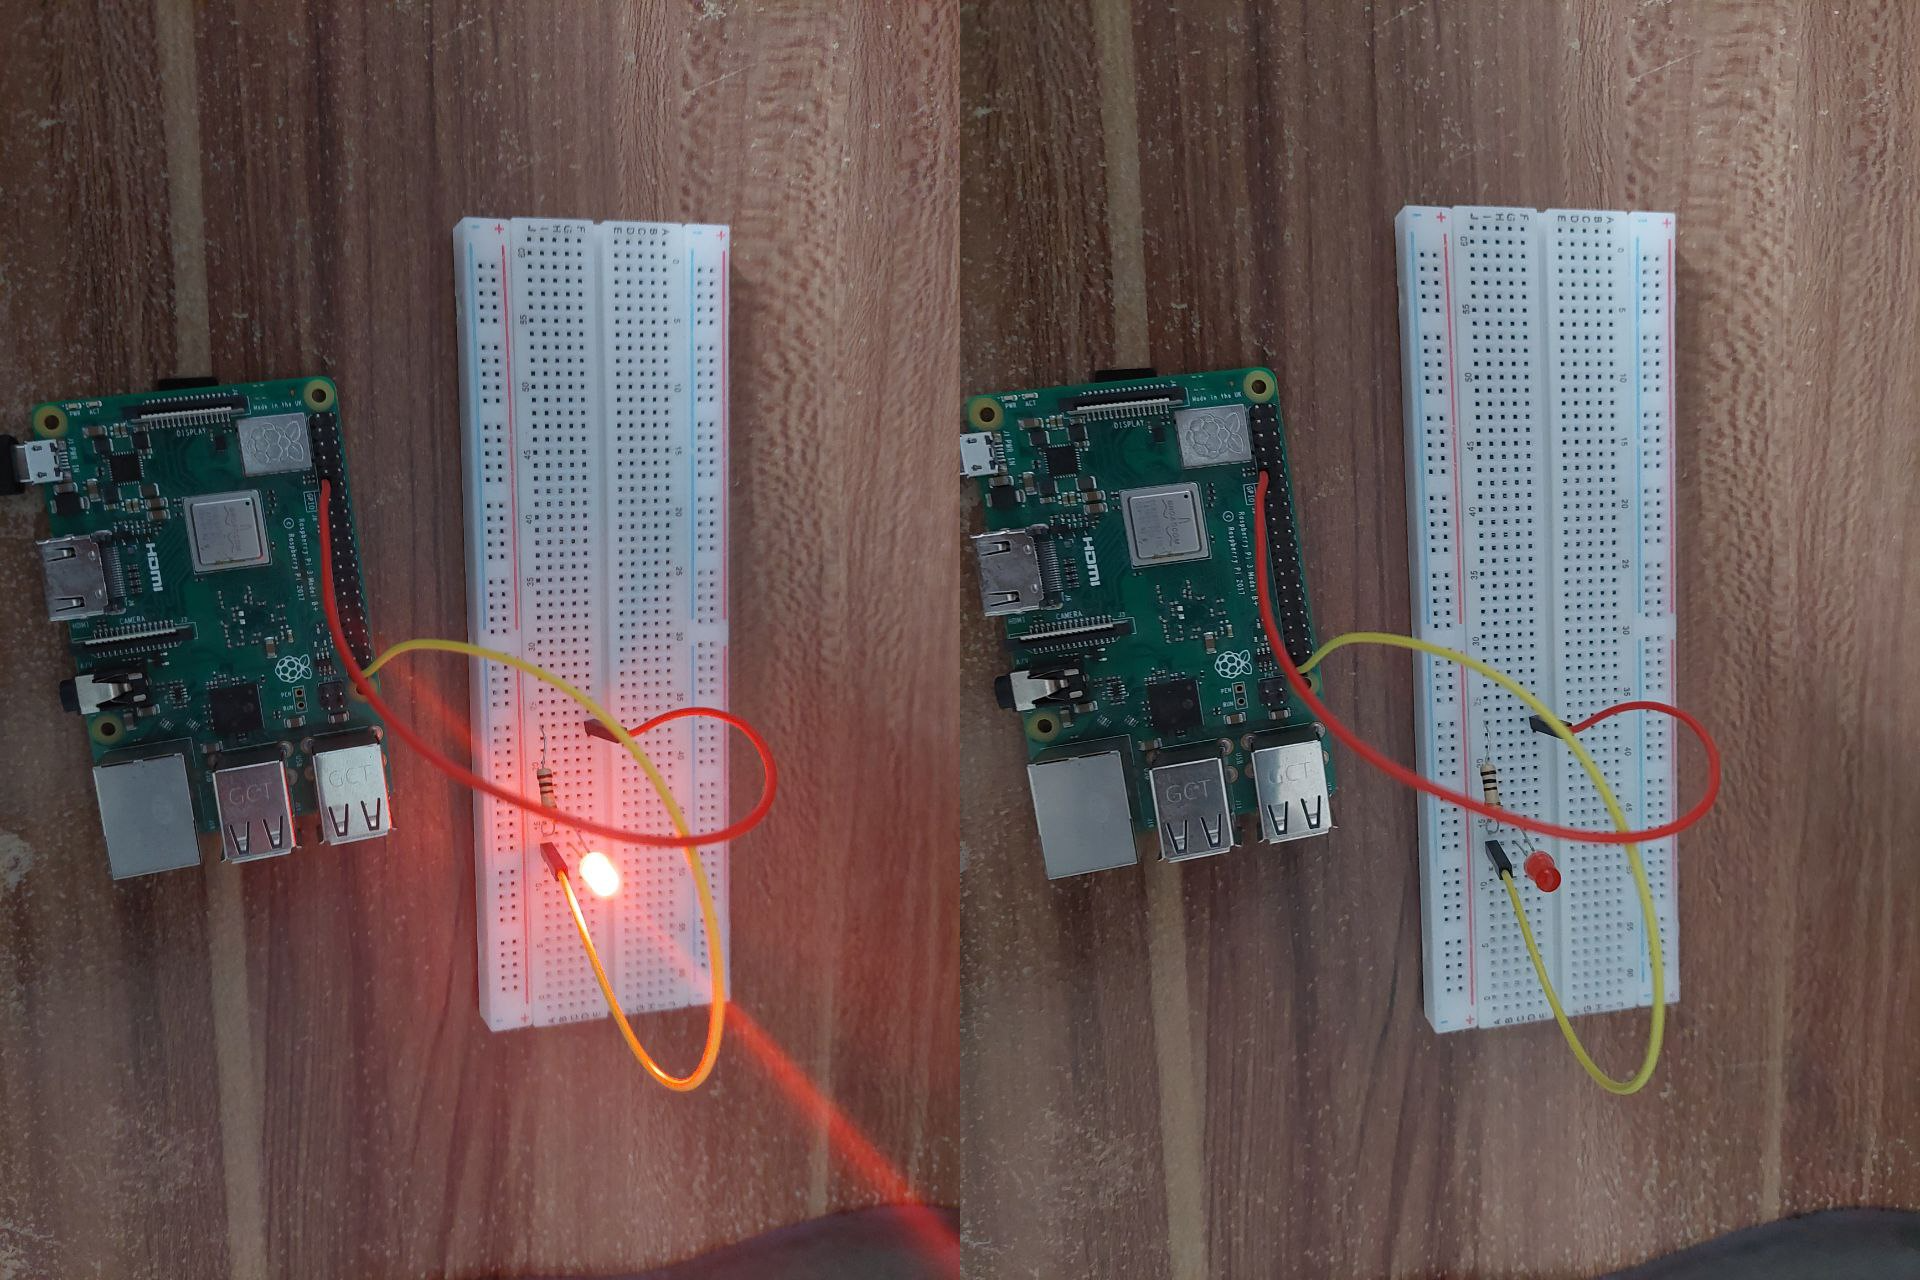
\includegraphics[scale=0.2]{new_update.png}
\caption{Successful firmware version update}
\label{new_update}
\end{figure}

In the test of the final version, it is required to have four files within the same directory: executable file, device certificate, device certificate private key, and device identity file. When the update is executed, the executable file is entirely replaced with the new update file. The files contained in the directory during the final execution can be seen in figure \ref{new_update}.

\begin{figure}[h]
\centering
\includegraphics[scale=1]{files_test.png}
\caption{Files contained in the project directory in final execution}
\label{new_update}
\end{figure}

\newpage

\renewcommand{\baselinestretch}{1.5} % line space
\section{Evaluation of the generic and scalable OTA architecture concept}

This section briefly describes the evaluation of the generic and scalable OTA architecture with the previous architectures. It is important to evaluate architecture in the early stages. The early the problem is realized, the better. It is cost-effective to fix errors in the requirements or early design phases compared to correcting them during the testing phase. An unsuitable architecture will cause disaster in a project. Along with that, performance and security goals will not be met. It will affect the schedules and budget of the project. Architecture is a project structure consisting of configurations, schedules and budgets, control libraries, performance and security goals, team structure, testing, maintenance, and documentation processes. If a single change is made in the architecture due to error, the entire project becomes chaotic. Thus, evaluating the architecture in the early stages of requirements and designing is important. \cite{r40} \\

The software industry came up with methods to evaluate software architectures in a standardized manner. There are many methods to evaluate architectures, but these methods, shown below, are widely used across the world:

\begin{itemize}
\item Architecture Trade-off Analysis Method (ATAS)
\item Software Architecture Analysis Method (SAAM)
\item Active Reviews for Intermediate Designs (ARID)
\end{itemize}

\subsection{Architecture Trade-off Analysis Method (ATAS)}

ATAS is a method for evaluating software architectures concerning the quality attribute goals. It exposes architectural failures and risks that can potentially harm an organization's achievements and business goals. Along with the exposure to risks, it gives insight into the quality of the goals - "how they trade off against each other". It is a leading method in the evaluation of software architecture. \cite{r39} \\

It is required for a complex software system to be a modifiable and good performance. It needs to be secure, portable, interoperable, and reliable. However, these qualities can sometimes be difficult to achieve for a particular set of systems. There are certain challenges: the precise meaning of these qualities for a particular system, analysis of desired qualities, time requirements for the analysis, and most importantly, knowing if the architecture is suitable without building the system first. Continuous efforts in designing are required to understand attributes and tackle challenges. \cite{r39} \\

The software architectures are built based on project decisions. First, scenarios are realized, and architectural decisions are made to support these scenarios. Then, scenarios and decisions are analyzed, and risk factors, non-risk factors, sensitivity points, and trade-off points are identified. Based on these risks, they are synthesized into risk themes, exposing the threats to the shareholder and business driver. This method consists of nine steps: \cite{r39} 

\begin{enumerate}

\item  \textbf{Present the ATAM}: It explains and sets expectations for the architecture. \cite{r39}
\item \textbf{Present business drivers}: The spoke-person of the project, usually the project manager or system customer, describes the business goals for the development efforts and primary architectural drivers, high availability, time to market, or high security. \cite{r39} 
\item \textbf{Present architecture}: The architecture designed by an architect. It addresses the relationship between architecture and business drivers. \cite{r39}
\item \textbf{Identify architectural approaches}: The approaches for the architecture are identified and defined. \cite{r39}
\item \textbf{Generate quality attribute utility tree}: The factors required in the system are performance, security, availability, re-usability, or modifiability. \cite{r39}
\item \textbf{Analyze architectural approaches}: Factors identified in the previous step are used to address and analyze architecture. Architectural risks, sensitivity points, and trade-offs are identified in this step. \cite{r39}

\item \textbf{Brainstorm and prioritize scenarios}: A set of scenarios is obtained from the group of stakeholders. It is prioritized usually through voting. \cite{r39}

\item \textbf{Analyze architectural approaches}: The scenarios are considered test cases to approve the performance of the analysis. It may uncover additional approaches, risks, sensitivity points, or trade-off points, which need to be documented. \cite{r39}

\item \textbf{Present results}: The analysis is presented to the stakeholders based on the information collected from the steps above. \cite{r39}

\end{enumerate}

This evaluation process helps identify risks early in the software development life-cycle, increases communication between stakeholders, clarifies quality attributes and requirements, and improves architecture documentation based on architectural decisions. \cite{r39}

\subsection{Software Architecture Analysis Method (SAAM)}

SAAM is an evaluation method that focuses on use cases. The evaluation structure structure consists of : \cite{r41}

\begin{enumerate}

\item Development of scenarios \cite{r41}
\item Describing candidate architecture \cite{r41}
\item Classification of scenarios \cite{r41}
\item Performing evaluation on scenarios \cite{r41}
\item Revealing scenario interaction \cite{r41}
\item Overall evaluation \cite{r41}

\end{enumerate}

Candidate architecture is the architecture that is chosen over other architectures. Describing the architecture is important, highlighting performance, parallel processing, task scheduling, communication, and modifiability issues. If additional views or attributes are needed, SAAM will clarify the requirements as it progresses. If two or more candidate architectures are evaluated, SAAM produces a ranking related to the candidates. SAAM points out the places or components that fail to meet the requirements if a single architecture is evaluated. Additionally, it shows better alternatives to the design in some cases. \cite{r41} \\

SAAM is a scenario-based method that characterizes the architectural design's responsiveness based on the demands of the set of scenarios. The scenario consists of a specified sequence of steps, which involves the use of the system modification. It serves as a representative for an entire set of scenarios. \cite{r41} 


\subsection{Active Reviews for Intermediate Designs (ARID)}

Both Active Reviews and ATAM are used to evaluate preliminary designs. Stakeholders receive detailed documentation of the architecture in the active design review. ATAM evaluates not only a portion of architecture but the whole architecture. ARID focuses on stakeholders and scenarios. It is an easy, light-weighted evaluation method, a combination of ATAM and Admission, Review, and Dismissal (ARD) methods. \cite{r42} \\

There are three roles in the ARID method: Facilitator, Scribe, and Questioners. The facilitator works with the architect in preparation for review meetings and facilitates all the architect's requirements. The scribe finds the issues and organizes review meetings to discuss issues. Questioners raise issues through questions and assist in scenario creation in the review meetings \cite{r42} \\

ARID is divided into two phases. In phase 1, the architect and review facilitators are in meetings. In the first step, the architect and facilitator identify a set of people for the review. In the next step, the design presentation is prepared, briefly explaining the design goals and details. In the next step, an initial scenario is prepared, illustrating the concept and architecture. In the final step of phase 1, the review meeting is conducted with the reviewers, and issues are discussed. After the end of phase 1, phase 2 begins. In the first step of phase 2, the ARID method is presented to the reviewers along with the necessary steps. In the next step, the design is presented, reviewers find issues in the design, and questioners ask questions and create scenarios to realize the architectural concept. In the next step, brainstorming is done on the architectural design, scenarios are prioritized, and architecture is changed accordingly. The next step is the review meeting to review the architecture after the discussed changes. These steps are repeated until the conclusion arrives. In the final step, the conclusion of the evaluation is presented to the reviewers, and voting is performed for the reviewers' opinions. \cite{r42}

\subsection{Evaluation for the generic and scalable architecture}

To evaluate the generic and scalable OTA architecture, ATAM is used since the steps involved in the ATAM evaluation method resemble the requirements for this Thesis. It involves identifying scenario-based criteria and an analysis of the architectural approaches. Approaching the architectural design is critical since it should match the design and security criteria. The generic and scalable OTA architecture is compared based on the earlier criteria. \cite{r43} \\

The criteria are based on scenarios considered throughout the Thesis. The analysis of design criteria can be seen below: 

\begin{itemize}

\item \textbf{User proximity}: From the cloud side, a supervising officer is required, responsible for certifications, cryptographic processes, and storing update files on the SFTP server. However, these processes can be performed remotely. On the other end, customers must be connected to the Internet to start the update process and can remotely monitor connected devices. It lowers user proximity significantly. 

\item \textbf{Latency and Jitter}: IoT devices are most likely connected to the Internet with a Wi-Fi router. Suppose many devices are connected to a single Wi-Fi router, and the latency and jitter increase. However, for a limited number of connected devices, the latency and jitter will not cause any issues to other processes running in the IoT device since the update process is performed as a separate task in the IoT device. Latency and jitter can also depend on the Internet plan and speed of the customer or the placement of IoT devices. 

\item \textbf{Network stability}: Network stability again depends on the placement and distance between the Wi-Fi router and IoT devices. However, the network will remain stable if the placement and internet plans are selected according to the needs. 

\item \textbf{High throughput}: The throughput also depends on the internet plan and placement. If the placement is wrong or the distance between the Wi-Fi router and IoT devices is significant, the latency increases and affects the network's throughput. Thus, correct placement of the IoT device is required to get high throughput. It also depends on the internet speed. The result below shows the time required to download file with a particular speed at consumer's scenario: \\

\begin{tabular}{ |p{3cm}||p{3cm}|p{3cm}|  }
\hline
 Download size& Download Speed & Elapsed time for download\\
 \hline
 100 MB   & 3.2 MB/s    & 28 sec. \\
 1 GB   & 3.6 MB/s    & 4 min. 49 sec. \\
 \hline
\end{tabular}


\item \textbf{Reliability}: If a service in the cloud or some component is not working correctly in the IoT device, the OEM will be notified within a specified time interval so that the necessary action can be taken as soon as possible. 

\item \textbf{Scalability}: IoT devices can be connected at ease. The customer needs all the certificates from the OEM, and the registration and connection process is automated. The number of connected devices can be either increased or decreased quickly according to the requirements. The services can be additionally assigned from the cloud side, and data can be routed easily. However, the services mentioned in the previous chapter should remain untouched. More services can be added, but the device manager, device provisioning, and SFTP server are necessary for the OTA update.

\item \textbf{Cost-efficient}: The high cost usually involves the purchase and maintenance of the server. However, the cloud solves that problem due to the pay-per-use program. The cloud providers only charge on the time the services are used.

\end{itemize}

The analysis based on the security can be seen below:

\begin{itemize}

\item \textbf{Authentication by design}: For the provisioning and registration of IoT devices, x509 certificates are used to authenticate the IoT device. It provides a high level of authentication security. These certificates are updated monthly so that the OEM can have control over their subscription service for the customers.

\item \textbf{Data confidentiality}: The update file is encrypted in two layers. Firstly, a 32-character hash key is generated and encrypted using the IoT device's public key, and the update file is encrypted using the hash key. The hash key is contained in a file. Both encrypted versions of the update file and hash key are uploaded to the SFTP server. The SHH connection must be established in the setup phase for the first time. Only the IoT device can access these files if the device is authenticated through SSH. The SSH authentication for the SFTP server is entirely separate from the authentication using certificates. Indeed, both of these authentications are required for the OTA update process. However, the SSH authentication is done for the first time during the setup phase, and the authentication through certificates should be down at the beginning of the program's execution.

\item \textbf{Data integrity}: Before uploading the file on the SFTP server, the checksum is generated. The checksum is a unique key linked to a file, and the checksum is provided to the IoT device as a desired property. Once the file is downloaded, the checksum is generated in the IoT device and is compared to the desired property. If it matches, the file is not tampered with or corrupted, and the decryption process can be performed. 

\end{itemize}


\newpage

\renewcommand{\baselinestretch}{1.5} % line space
\section{Conclusion and future work}

The prototype was implemented and executed with successful results. Due to the evaluation based on criteria in the previous chapter, the OTA update system architecture has a high level of scalability due to automatic provisioning and is generic. The OTA update system architecture can be applied to any IoT device. However, it is required to have a Software Development Kit (SDK) as middleware on top of the application program. The SDK connects the cloud and the application running program. Depending on the type of IoT device, the SDK requirement changes. It might be possible that different variants of SDKs are used to run application programs in a different types of IoT devices. In general, the cloud-based OTA update system architecture is generic and scalable. \\

The work shown in this thesis exists in the OTA update system's design and evaluation scope. From the cloud perspective, additional services can be added:

\begin{itemize}

\item \textbf{Data analytics}: Data analytic services can be used to analyze the telemetry data from the sensors to generate data sets and find information in the data sets. Additional services can be added to realize insights into the data.

\item \textbf{Event trigger using smart device}: A smart device can be used to trigger necessary events and run queries. It can also be used to add, modify, or delete several IoT devices' configurations. REST API can be used to send requests to the cloud with the payload containing the information, and the cloud acts upon it. It can either be a mobile application or website, through which the configuration can be changed, or an event can be triggered. It is helpful for the customer as well as OEM.

\item \textbf{Version Management}: In this thesis, version management was considered out of the scope. However, it is an essential part of the OTA update process. In case of failure during the installation of the new update, it is required to revert to the previous version. Researchers have found methods to resolve the issue. However, these methods are not profound and need thorough research on the best possible method considering the advantages and disadvantages.

\end{itemize}



\newpage


\raggedright

\newpage                                                                                %biblography
%\section{Reference}
\begin{thebibliography}{}

\bibitem{r1} 
Smith, J., 2022. Was ist ein Over-the-Air-Update?. [Blog] Computerwoche, Available at: \url{https://www.computerwoche.de/a/was-ist-ein-over-the-air-update,3551551} [Accessed 9 May 2022]. 

\bibitem{r2}
Debauche, O., Mahmoudi, S., Manneback, P. and Lebeau, F., 2021. Cloud and distributed architectures for data management in agriculture 4.0 : Review and future trends. Journal of King Saud University - Computer and Information Sciences, [online] Available at: \url{https://www.sciencedirect.com/science/article/pii/S1319157821002664} [Accessed 13 May 2022].

\bibitem{r3}
Steger, M., Karner, M., Hillebrand, J., Rom, W., Boano, C. and Römer, K., 2016. Generic framework enabling secure and efficient automotive wireless SW updates. Institute for Technical Informatics, Graz University of Technology, Graz, Austria, [online] Available at: \url{http://www.carloalbertoboano.com/documents/steger16generic.pdf} [Accessed 13 May 2022].

\bibitem{r4}
Jyotsna, 2021. 12 Major Applications of IoT You Should Know | Jigsaw Academy. [online] Jigsaw Academy. Available at: \url{https://www.jigsawacademy.com/top-uses-of-iot/} [Accessed 9 May 2022].

\bibitem{r5}
Driver, C., 2018. How to Approach OTA Updates for IoT. [Blog] Medium, Available at: \url{https://medium.com/@temboo/how-to-approach-ota-updates-for-iot-d088c217b31c} [Accessed 9 May 2022].

\bibitem{r6}
Halder, S., Ghosal, A. and Conti, M., 2020. Secure over-the-air software updates in connected vehicles: A survey. Computer Networks, [online] 178, p.107343. Available at: \url{https://arxiv.org/pdf/1904.00685.pdf} [Accessed 10 May 2022].

\bibitem{r7}
HARMAN Automotive. n.d. How can OTA be a revenue generator for agricultural machinery manufacturer?. [online] Available at: \url{https://car.harman.com/insights/articles/how-are-agricultural-vehicles-updated-with-ota-solutions} [Accessed 9 May 2022].

\bibitem{r8}
Smart-AKIS. n.d. What is Smart Farming? - Smart-AKIS. [online] Available at: \url{https://www.smart-akis.com/index.php/network/what-is-smart-farming/} [Accessed 11 May 2022].

\bibitem{r9}
Venki, V., 2018. What is the OTA update for smartphones?. [online] Quora. Available at: \url{https://www.quora.com/What-is-the-OTA-update-for-smartphones} [Accessed 11 May 2022].

\bibitem{r10}
HARMAN Digital Transformation Solutions, 2017. Over-the-Air (OTA) Updates Empower Intelligent Gadgets to Continually Evolve. Available at: \url{https://services.harman.com/blogs/harman-ota-empowers-intelligent-gadgets-move-beyond-merely-solving-problems} [Accessed 11 May 2022].

\bibitem{r11}
Cai, H., Jiang, L. \& Chao, KM. Current and future of software services in smart manufacturing. SOCA 14, 75–77 (2020). Available at: \url{https://doi.org/10.1007/s11761-020-00293-y} [Accessed 27 May 2022]

\bibitem{r12}
Luber, S. and Litzel, N., 2017. Was ist ein Cyber-physisches System (CPS)?. [online] Bigdata-insider.de. Available at: \url{https://www.bigdata-insider.de/was-ist-ein-cyber-physisches-system-cps-a-668494/} [Accessed 28 May 2022].

\bibitem{r13}
Villegas, M., Orellana, C. and Astudillo, H., 2019. A study of over-the-air (OTA) update systems for CPS and IoT operating systems. Proceedings of the 13th European Conference on Software Architecture - ECSA '19 - volume 2, [online] Available at: \url{https://www.researchgate.net/publication/335641549_A_study_of_over-the-air_OTA_update_systems_for_CPS_and_IoT_operating_systems} [Accessed 28 May 2022].

\bibitem{r14}
Ranger, S., 2022. What is cloud computing? Everything you need to know about the cloud explained. [online] ZDNet. Available at: \url{https://www.zdnet.com/article/what-is-cloud-computing-everything-you-need-to-know-about-the-cloud/} [Accessed 30 May 2022].

\bibitem{r15}
cloudflare. n.d. What is the cloud?. [online] Available at: \url{https://www.cloudflare.com/learning/cloud/what-is-the-cloud/} [Accessed 30 May 2022].

\bibitem{r16}
Greer, C., Griffor, E., Burns, M. and Wollman, D., 2017. The Intersection of IoT and CPS. [ebook] National Institute of Standards and Technology. Available at: \url{http://www.picasso-project.eu/wp-content/uploads/2017/06/2017-06-19-9h15_Keynote_Greer.pdf} [Accessed 31 May 2022].

\bibitem{r17}
Rizal, D., 2020. Software Architecture and Design. [online] Medium. Available at: \url{https://medium.com/the-legend/software-arsitektur-dan-design-90f76288078e} [Accessed 31 May 2022].

\bibitem{r18}
Richards, M., 2015. Software Architecture Patterns. 1st ed. CA,USA : O'Reilly Media, Inc.

\bibitem{r19}
Ozkaya, M., 2021. Service-Oriented Architecture. [Blog] medium, Available at: \url{https://medium.com/design-microservices-architecture-with-patterns/service-oriented-architecture-1e4716fbca17} [Accessed 1 June 2022].

\bibitem{r20}
Afreen, S., 2022. What Is Cloud Computing Architecture: Benefits, Components \& More [Blog] simplilearn, Available at: \url{https://www.simplilearn.com/tutorials/cloud-computing-tutorial/cloud-computing-architecture} [Accessed 1 June 2022].

\bibitem{r21}
Javatpoint. 2022. Cloud Computing Architecture - javatpoint. [online] Available at: \url{https://www.javatpoint.com/cloud-computing-architecture} [Accessed 1 June 2022].

\bibitem{r22}
Scheible, T., n.d. IT-Sicherheit Grundlagen: Schutzziele. [online] Scheible.it. Available at: \url{https://scheible.it/it-sicherheit-grundlagen-schutzziele/} [Accessed 7 June 2022].

\bibitem{r23}
Tutorialspoint.com. n.d. Cryptography Tutorial. [online] Available at: \url{https://www.tutorialspoint.com/cryptography/index.htm} [Accessed 21 June 2022].

\bibitem{r24}
Cheah, D., 2019. Basics of Cryptography. [online] Medium. Available at: \url{https://medium.com/@tattwei46/basics-of-cryptography-18d01b952dde} [Accessed 21 June 2022].

\bibitem{r25}
Krishnan, M., 2019. Architectural patterns for the Cloud - Mahesh Krishnan. [online] Youtube.com. Available at: \url{https://www.youtube.com/watch?v=TuZZIGSbFfQ} [Accessed 27 June 2022].

\bibitem{r26}
Flower, Z., 2021. 5 cloud design patterns to create resilient applications. [online] SearchCloudComputing. Available at: \url{https://www.techtarget.com/searchcloudcomputing/tip/5-cloud-design-patterns-to-create-resilient-applications} [Accessed 27 June 2022].

\bibitem{r27}
Lethaby, N., 2018. A more secure and reliable OTA update architecture for IoT devices. [ebook] Texas Instruments. Available at: \url{https://www.ti.com/lit/wp/sway021/sway021.pdf?ts=1656579651621&ref_url=https%253A%252F%252Fwww.google.com%252F} [Accessed 30 June 2022].

\bibitem{r28}
Guissouma, H., 	Diewald, A., Sax, E., 2018. A Generic System for Automotive Software Over The Air (SOTA) Updates Allowing Efficient Variant and Release Management [ebook] Springer International Publishing. Available at: \url{https://www.springerprofessional.de/en/a-generic-system-for-automotive-software-over-the-air-sota-updat/16079956} [Accessed 13 July 2022].

\bibitem{r29}
Hong S., Kim N. and Heo T., 2015. A smartphone connected software updating framework for IoT devices. 2015 International Symposium on Consumer Electronics (ISCE), [online] Available at: \url{https://ieeexplore.ieee.org/document/7177805} [Accessed 21 July 2022].

\bibitem{r30}
Chandra, H., Anggadjaja, E., Wijaya, P. and Gunawan, E., 2016. Internet of Things: Over-the-Air (OTA) firmware update in Lightweight mesh network protocol for smart urban development. 2016 22nd Asia-Pacific Conference on Communications (APCC), [online] Available at: \url{https://ieeexplore.ieee.org/document/7581459} [Accessed 24 July 2022].

\bibitem{r31}
Chandra, H., Anggadjaja, E., Wijaya, P. and Gunawan, E., 2016. Internet of Things: Over-the-Air (OTA) firmware update in Lightweight mesh network protocol for smart urban development. 2016 22nd Asia-Pacific Conference on Communications (APCC), [online] Available at: \url{https://ieeexplore.ieee.org/document/7581459} [Accessed 24 July 2022].

\bibitem{r32}
Gumel, M., Faruk, N., 2020. Wireless mesh network throughput capacity analysis. Faculty of Engineering and technology, University of Ilorin, Ilorin, Nigeria, [online] Available at: \url{https://www.researchgate.net/publication/295403088_WIRELESS_MESH_NETWORKS_THROUGHPUT_CAPACITY_ANALYSIS} [Accessed 7 August 2022].

\bibitem{r33}
Brush, K., Rosencrance, L. and Cobb, M., 2021. What is Asymmetric Cryptography? Definition from SearchSecurity. [online] SearchSecurity. Available at: \url{https://www.techtarget.com/searchsecurity/definition/asymmetric-cryptography} [Accessed 12 August 2022].

\bibitem{r34}
Thales Group. 2022. 5G technology and networks (speed, use cases, rollout). [online] Available at: \url{https://www.thalesgroup.com/en/markets/digital-identity-and-security/mobile/inspired/5G} [Accessed 15 August 2022].


\bibitem{r35}
Quora. n.d. What do you do when you have too many devices on WiFi?. [online] Available at: \url{https://www.quora.com/What-do-you-do-when-you-have-too-many-devices-on-WiFi} [Accessed 16 August 2022].

\bibitem{r36}
Docs.microsoft.com. n.d. Developer tools, technical documentation and coding examples. [online] Available at: \url{https://docs.microsoft.com/} [Accessed 31 August 2022].

\bibitem{r37}
2022. What is SFTP Server - Ipswitch. [online] Available at: \url{https://www.ipswitch.com/resources/best-practices/sftp-server} [Accessed 4 September 2022].


\bibitem{r38}
Krohn, M., 2022. What is MQTT? A practical introduction. [online] System integration with the OPC Router. Available at: \url{https://www.opc-router.com/what-is-mqtt/} [Accessed 5 September 2022].

\bibitem{r39}
Resources.sei.cmu.edu. n.d. Architecture Tradeoff Analysis Method Collection. [online] Available at: \url{https://resources.sei.cmu.edu/library/asset-view.cfm?assetid=513908} [Accessed 9 September 2022].

\bibitem{r40}
Pearsonhighered.com. n.d. [online] Available at: \url{https://www.pearsonhighered.com/assets/samplechapter/0/2/0/1/020170482X.pdf} [Accessed 10 September 2022].

\bibitem{r41}
Kommadi, B., 2020. SAAM : Software Architecture Analysis Method. [online] Medium. Available at: \url{https://medium.com/@bhagvankommadi/saam-software-architecture-analysis-method-36864cd8ea94} [Accessed 10 September 2022].

\bibitem{r42}
GeeksforGeeks. 2020. Active Reviews for Intermediate Designs (ARID) in Software Architectures - GeeksforGeeks. [online] Available at: \url{https://www.geeksforgeeks.org/active-reviews-for-intermediate-designs-arid-in-software-architectures/} [Accessed 10 September 2022].

\bibitem{r43}
Bridges, D., 2015. Methods and Models for Evaluating Software Product Line Architecture Hyotaeg Jung Computer Science Department Univ. of Texas at Dallas Software Architecture. - ppt download. [online] Slideplayer.com. Available at: \url{https://slideplayer.com/slide/5966216/} [Accessed 11 September 2022].

\bibitem{r44}
TechVidvan. n.d. IoT Hardware Devices. [online] Available at: \url{https://techvidvan.com/tutorials/iot-hardware/} [Accessed 13 September 2022].

\bibitem{r45}
Youtube. 2020. Enrollment Groups with Azure Device Provisioning Service. [online] Available at: \url{https://www.youtube.com/watch?v=9XlhuqtQ7kk&t=766s} [Accessed 14 September 2022].

\bibitem{r46}
Cpl.thalesgroup.com. n.d. Hardware Security Modules (HSMs) | Thales. [online] Available at: \url{https://cpl.thalesgroup.com/encryption/hardware-security-modules} [Accessed 15 September 2022].

\bibitem{r47}
GitHub. n.d. Implementing A Custom HSM [online] Available at: \url{https://github.com/Azure/azure-iot-sdk-c/blob/main/provisioning_client/devdoc/using_custom_hsm.md} [Accessed 15 September 2022].

\bibitem{r48}
Awati R., 2021. What is a cryptographic checksum and does it verify files? [online] Available at: \url{https://www.techtarget.com/searchsecurity/definition/cryptographic-checksum} [Accessed 18 September 2022].


\end{thebibliography}

\newpage
\section*{Plagiarism Declaration}

I, \textbf{Prithvi Patel}, hereby certify that the thesis on \textbf{Analysis and evaluation of needs for a generic and scalable cloud-based OTA update system} is solely my work, and I have only used the sources stated in the reference section. Each portion of my thesis containing external sources, which includes electronic media, and direct or indirect quotations, have been acknowledged as such and sources cited. \\


\vspace{1cm}
\vspace{1cm}
\noindent\begin{tabular}{@{}p{2.5in}p{1in}p{2.5in}@{}}
\dotfill                        & & \dotfill\\
Prithvi Patel             & & Date\\
RWU University of Applied Science  
                           &      & \\[8ex]

\end{tabular} 



\clearpage

\end{document}
